\documentclass{scrartcl}

\usepackage[T1]{fontenc}
\usepackage[utf8]{inputenc}

\usepackage{amsmath}
\usepackage{amssymb}
\usepackage{array}
\usepackage{authblk}
   \renewcommand\Affilfont{\small}
   \renewcommand{\Authsep}{\\}
   \renewcommand{\Authand}{\\}
   \renewcommand{\Authands}{\\}
\usepackage[ngerman]{babel}
\usepackage[natbib,notes,backend=bibtex,url=true]{biblatex-chicago}
   \bibliography{references}
\usepackage{booktabs}
\usepackage{caption}
\usepackage[german=guillemets]{csquotes}
\usepackage{dcolumn}
   \newcolumntype{d}[1]{D{.}{.}{#1}}
\usepackage{fbox}
   \setlength{\fboxsep}{0pt}
   \setlength{\fboxrule}{1pt}
\usepackage{float}
\usepackage{graphicx}
   \setkeys{Gin}{width=\linewidth,totalheight=\textheight,keepaspectratio}
   \graphicspath{{figures/}}
\usepackage[hidelinks]{hyperref}
   \urlstyle{rm}
\usepackage{longtable}
\usepackage{pdflscape}
\usepackage{xcolor}
\usepackage{xurl}

\newcolumntype{L}[1]{>{\raggedright\arraybackslash}p{#1}}

\deffootnote{1.5em}{1em}{\makebox[1.5em][l]{\thefootnotemark}}
   \setlength{\skip\footins}{1.5em}
   \setlength{\footnotesep}{1em}

\title{\enquote{Einhundert Leute\\haben wir gefragt~$\ldots$}}
\subtitle{Einblicke in Methodenvielfalt und Interdisziplinarität\\der Game Studies im deutschsprachigen Raum}

\author[1]{Alexander Max Bauer}
\author[2]{Lukas Daniel Klausner}
\author[3]{Tobias Unterhuber}

\affil[1]{ Carl von Ossietzky Universität Oldenburg, Institut für Philosophie}
\affil[2]{ Fachhochschule St. Pölten, Institut für IT Sicherheitsforschung}
\affil[3]{ Universität Innsbruck, Institut für Germanistik}

\date{}


\begin{document}
\maketitle
\thispagestyle{empty}

\begin{center}
   \textbf{\textsf{in Vorbereitung für:}}\\
   Alexander Max Bauer, David Betzing, Jacob Birken, Simon Hagemann, Lukas Daniel Klausner, Alina Menten, Christian Sturm und Tobias Unterhuber (Hrsg.): \textit{Geisteswissenschaften und Digitale Spiele. Debatten, Data \& Desiderata}.
\end{center}

\vfill
\noindent\textbf{\textsf{Abstract:}}
Die Game Studies sind als junges und inhärent interdisziplinäres Feld auch selbst ein hochgradig interessanter Forschungsgegenstand.
Vor diesem Hintergrund untersucht unser Beitrag Methodenvielfalt und disziplinäre Verortung der Game Studies im deutschsprachigen Raum, wobei auch der Kontrast zur Situation im englischsprachigen bzw. internationalen Kontext reflektiert wird.
Ausgangspunkt ist eine Online-Umfrage unter Forschenden ($n = 100$), ergänzt um theoretische Überlegungen zur Frage, wie sich das Feld zwischen Disziplinarität und Interdisziplinarität positioniert.
Um die doppelte Verortung der Game Studies zwischen Ursprungsdisziplin und Forschungsfeld zu beschreiben, schlagen wir den Begriff der disziplinären Affordanz vor.
Unsere Umfrageergebnisse liefern Daten zur Geschlechter-, Alters- und Fächerverteilung in den deutschsprachigen Game Studies.
Darüber hinaus zeigen sie, dass die Methoden- und Theoriewahl in den Game Studies stark von den jeweiligen Ursprungsdisziplinen der Forschenden geprägt sind.
Ausgehend von diesen Ergebnissen werden Problemfelder und Handlungsempfehlungen vorgeschlagen.


%%%%%%%%%%%%%%
% EINLEITUNG %
%%%%%%%%%%%%%%
\newpage
\section{Einleitung}\label{sec:einleitung}
Es gibt kaum ein Forschungsfeld, das so interdisziplinär ist wie die Game Studies.
Okay, das ist zweifelsohne in dieser starken Formulierung Unfug, aber die Beforschung Digitaler Spiele ist tatsächlich einer der hochgradig interdisziplinären Wissenschaftszweige im akademischen Betrieb.
Was die Game Studies vielleicht tatsächlich auszeichnet, ist, dass sich bislang (mutmaßlich auch wegen ihrer relativen Jugend)\autocite[Vgl.][]{unterhuber_magic_2022} noch kein wirklicher Methoden- oder Theoriekanon herausgebildet zu haben scheint.
Vor diesem Hintergrund wollen wir das Jubiläum des Arbeitskreises zum Anlass nehmen, uns ausführlich und datenbasiert mit den gängigen Methoden und der disziplinären Verortung der Game-Studies-Forscher:innen im deutschen Sprachraum zu befassen.
Im Folgenden werfen wir hierzu zunächst einen Blick auf den theoretischen Hintergrund (\autoref{sec:hintergrund}), ehe wir die von uns durchgeführte Umfrage vorstellen (\autoref{sec:methodik}) und einen eingehenden Blick auf ihre Ergebnisse werfen (\autoref{sec:resultate}).
Zum Abschluss versuchen wir, unsere Erkenntnisse noch einmal gesammelt zu interpretieren und in einen breiteren Kontext zu stellen (\autoref{sec:conclusio}).


%%%%%%%%%%%%%%%
% HINTERGRUND %
%%%%%%%%%%%%%%%
\section{Theoretischer Hintergrund}\label{sec:hintergrund}
Zunächst aber steht die Frage im Raum, als was die Game Studies am besten zu verstehen sind:
Sind sie eine Disziplin oder doch eher ein Feld?\footnote{Foucault beispielsweise versteht unter Disziplinen \enquote{Gesamtheiten von Aussagen [$\ldots$], die ihre Organisation wissenschaftlichen Modellen entleihen, zur Kohärenz und zur Beweisfähigkeit neigen, wie Wissenschaften angenommen, institutionalisiert, übermittelt und manchmal gelehrt werden} (\autocite[][S.~253--254]{foucault_archaologie_2011}). Forschungsfelder hingegen fungieren begrifflich vor allem als Gegenstandsbereich ohne Notwendigkeit einer institutionellen Grundlage.}
Wie an anderer Stelle bereits angemerkt, scheint es den Game Studies (oder der Spielwissenschaft oder der Spielforschung) im deutschsprachigen Raum an Institutionalisierung und somit an stabilisierender Verankerung zu fehlen,\autocite[Vgl.][S.~26]{unterhuber_wer_2024} so dass \enquote{sich von den Game Studies am besten als Feld sprechen} lässt.\autocite[][S.~26]{unterhuber_wer_2024}
Damit werden aber auch die Ursprungsdisziplinen der einzelnen Forscher:innen wichtiger -- \enquote{Computerspiele werden von den verschiedensten Disziplinen aus beforscht und hieraus ergeben sich fruchtbare Synergien und eine grundlegende Multiperspektivität}.\footnote{\autocite[][S.~26]{unterhuber_wer_2024}; siehe zur konkreten inter- und multidisziplinären Zusammenarbeit über Fachgrenzen hinweg auch den Erfahrungsbericht aus dem Schweizer Confoederatio-Ludens-Projekt: \autocite{bemelmans_bridging_2024}.}
Damit einher geht, so unsere Vermutung, auch eine Vielzahl verschiedener Ansätze, Methoden und Theorien.
Aber was hat das wiederum für eine Auswirkung auf die Game Studies?
Welche Rolle spielen gemeinsame Methoden und Theorien für das Feld?

Oliver Jahraus folgend werden Fächer (und wohl auch Felder) nicht nur durch ihre Gegenstände und ihre Zugänge zu diesen definiert, sondern auch durch die komplexen und spezifischen Relationen zwischen diesen beiden Polen, die zu einer doppelseitigen Objektkonstitution führen.\autocite[Vgl.][S.~6]{jahraus_literaturtheorie_2004}
Foucaults Verständnis von der Disziplin eines Diskurses \enquote{definiert sich durch einen Bereich von Gegenständen, ein Bündel von Methoden, ein Korpus von als wahr angesehenen Sätzen, ein Spiel von Regeln und Definitionen, von Techniken und Instrumenten}.\autocite[][S.~22]{foucault_ordnung_1993}
Die Disziplin fungiert als \enquote{Kontrollprinzip der Produktion des Diskurses} und setzt damit die \enquote{Grenzen [des Diskurses] durch das Spiel einer Identität, welche die Form einer permanenten Reaktualisierung der Regeln hat}.\autocite[][S.~25]{foucault_ordnung_1993}
Die Regeln der Sagbarkeit eines Diskurses und somit einer Disziplin, auch im wissenschaftlichen Sinne, funktionieren also als soziokulturelle und diskursive Praxis durch das Zusammenspiel von formalen, sozialen, internen, externen und materiellen Regeln und sind somit dem Spiel ähnlich -- oder zumindest als spielförmig erfassbar --,\footnote{\autocite[Vgl.][S.~2--3]{stenros_rule_2024}; \autocite[][S.~24--325]{unterhuber_spielgeschichten_nodate}} auch wenn nicht alle Beteiligten, abhängig von z.\,B. ihrem Status, den gleichen Regeln unterliegen.
Zu einer ähnlichen Anschauung kommt auch Daniel Wrana, wenn er den Widerstreit verschiedener Disziplinen \enquote{im Terrain des \enquote{eigentlichen} wissenschaftlichen Spiels} um \enquote{Methodologien und um intellektuelle Techniken} untersucht:\autocite[][S.~49]{wrana_inter-disziplinaritat_2017}

\begin{quote}
   Jede dieser Äußerungen ist zugleich ein Spielzug in einem diskursiven Kampf, ob der Spielzug \enquote{gelingt}, ob sich also das Terrain in der Weise strukturiert, wie im Spielzug postuliert wird, ist nie ganz vorhersehbar, sondern Resultat eines komplexen Spiels von Ereignissen und Kräfteverhältnissen.
   Jede Äußerung ist demzufolge im vollen Sinn ein Einsatz im Spiel, sie ist ein Claim für eine Position im umkämpften Terrain.\autocite[][S.~43]{wrana_inter-disziplinaritat_2017}
\end{quote}

Somit können Disziplinen, Fächer, Felder also auch als Spiele, die wiederum im größeren wissenschaftlichen Spiel mit anderen konkurrieren (oder zusammenarbeiten oder, neutraler gewendet, interagieren), verstanden werden.
Die Disziplin eines Diskurses formt damit sowohl die Außenwahrnehmung als auch die Selbstwahrnehmung.
Wrana betont dabei, dass es vor allem auch \enquote{die Formierung von Begriffen und Methoden} ist, die zur Definition von Disziplinen und vor allem von \enquote{disziplinären Grenzen} beiträgt und dass diese am besten als \enquote{durch Machtverhältnisse hervorgebracht und von Machtverhältnissen durchzogen zu verstehen} seien.\autocite[][S.~45]{wrana_inter-disziplinaritat_2017}
Oder wie Bettina Beer und Matthias Koenig formulieren:
\enquote{Disziplinen differenzieren sich nicht naturwüchsig, sondern als Ergebnis strategischer Praktiken der Grenzziehung.}\autocite[][S.~4]{beer_grenzziehungen_2009}
Diese \enquote{Erkenntnispolitik}\footnote{\autocite[][S.~115--121]{seitter_erkenntnispolitik_1985}; \autocite[][S.~45]{wrana_inter-disziplinaritat_2017}.} zeigt auch auf, dass sich eine Trennung zwischen diesen Aushandlungen und der \enquote{eigentliche[n] wissenschaftlich-fachliche[n] Debatte [$\ldots$] kaum halten} lässt:\autocite[][S.~49]{wrana_inter-disziplinaritat_2017}

\begin{quote}
   Vielmehr setzen sich die diskursiven Kämpfe im Terrain des \enquote{eigentlichen} wissenschaftlichen Spiels fort, hier wird um Methodologien und um intellektuelle Techniken gekämpft und damit auch um differente Gegenstandsformierungen und den legitimen bzw. exklusiven Zugriff auf Gegenstandsbereiche und diese werden wiederum zu Mitteln im Kampf um disziplinäre Grenzen und Ressourcen.
   Gegenstände und Techniken werden zu Einsätzen im doppelten Sinn: sie sind umkämpftes Gut und zugleich ein Mittel im Kampf.\autocite[][S.~49--50]{wrana_inter-disziplinaritat_2017}
\end{quote}

Sabine Hark begreift in ihren Ausführungen zur Fachwerdung der Gender Studies Anfang der $2000$er die wissenschaftliche Disziplin als \enquote{eine der wichtigsten} Spielregeln im wissenschaftlichen Feld.\autocite[][S.~96]{hark_diszipliniertes_2001}
Nun ist es aber eine Besonderheit, dass es im deutschsprachigen Raum eben -- noch (?) -- keine Disziplin \enquote{Game Studies} gibt.\autocite[Vgl.][S.~96]{rautzenberg_spielformige_2021}
Vielmehr stammen alle Wissenschaftler:innen eigentlich aus anderen Disziplinen -- mit ihren jeweils eigenen Regeln und Selbstverständnissen.
Martin Guntau und Hubert Laitko haben in ihrer großen Studie zur Entstehung moderner wissenschaftlicher Disziplinen festgestellt, dass \enquote{Disziplinbindung [$\ldots$] ein Persönlichkeitsmerkmal} sei,\autocite[][S.~12]{guntau_einleitung_2021} das die Sicht der Einzelpersonen nachdrücklich mitbestimmt.
Was aber passiert, wenn man sich aus dieser disziplinären Position einem neuen Gegenstand, wie dem Videospiel, widmet?
Welcher Blickwinkel wird den Wissenschaftler:innen von ihren Ursprungsdisziplinen auferlegt?

Mag durch das Voranschreiten der Interdisziplinarität mittlerweile heutzutage keine \enquote{wissenschaftliche Ausbildung nur eine monodisziplinäre Qualifikation im engen Sinne des Wortes vermitteln}, ist dennoch \enquote{die Stammdisziplin [$\ldots$] der systembildende Faktor, der die Beiträge der anderen Disziplinen integriert und das Verhältnis des werdenden Wissenschaftlers zu diesen vorprägt}.\autocite[][S.~13]{guntau_einleitung_2021}
Um genau diesen \enquote{systembildenden Faktor}, der auch mit diskursiven Praktiken verknüpft ist, geht es uns.
Unsere Annahme ist es, dass bei der Erweiterung eines Gegenstandsbereichs einer Disziplin oder beim Sich-Begeben auf transdisziplinäres Terrain sonst nicht mehr wirksame Mechanismen der jeweiligen wissenschaftlichen Disziplin in Kraft gesetzt werden.\footnote{Thomas S. Kuhn widmet sich zwar ausführlich der Veränderung von Wissenschaften unter dem Stichwort des Paradigmenwechsels und der Wandlung des Weltbildes, beobachtet dabei aber vor allem, wie sich durch neue Erkenntnisse, Methoden, Zugänge etc. die Sicht der Wissenschaftler:innen ändert, nicht aber, wie diese Veränderung von anderen wahrgenommen wird (\autocite[vgl.][]{kuhn_struktur_1997}). Auch wäre der Begriff des \enquote{Paradigmas} wohl zu viel des Guten, geht es hier ja nicht um eine komplette Umformung einer existierenden Disziplin, sondern um entweder eine Erweiterung der Gegenstandsbereiche oder die Beteiligung an einem transdisziplinären Feld, das selbst wiederum Disziplin werden könnte. Auch der schwächere Begriff des \enquote{Turns}, der \enquote{a shift in perspective, an opportunity to view a yet-unseen facet of a problem} impliziert (\autocite[][S.~7]{meierhofer_turns_2011}), scheint unpassend -- auch wenn die Reaktionen auf die diversen Trends der letzten Jahrzehnte z.\,B. in den Literaturwissenschaften eine ähnlich drastische Abneigung gegenüber allem Neuen an den Tag legen (\autocite[vgl. auch][S.~9--22]{sturm-trigonakis_turns_2017}). Gerade auch die von uns im folgenden angeschnittene Frage nach der (disziplinären) Eigenständigkeit der spielwissenschaftlichen Methoden- und Theoriebildung zeigt, dass es sich eben nicht um einen Turn handelt: \enquote{Von einem \textit{turn} kann man erst sprechen, wenn der neue Forschungsfokus von der Gegenstandsebene neuartiger Untersuchungsfelder auf die Ebene von Analysekategorien und Konzepten \enquote{umschlägt}, wenn er also nicht mehr nur neue Erkenntnis\textit{objekte} ausweist, sondern selbst zum Erkenntnis\textit{mittel} und -\textit{medium} wird} (\autocite[][S.~26]{bachmann-medick_cultural_2006}; Hervorhebung im Original).}
Das Fach \enquote*{fordert} aufgrund der freieren Regelauslegung, auch Spiel als Gegenstand zu begreifen, andere Aspekte der Disziplin umso härter umzusetzen.
Dies betrifft vor allem die theoretischen und methodischen Zugänge, aber auch Formen der Arbeitsweisen und die Rahmung des Gegenstands als Gegenstand.
Dabei scheint es nur schwer möglich, die eigentlichen State-of-the-Art-Ansätze der eigenen Disziplin zu bemühen, sondern es werden erprobte und vielleicht sogar angestaubte \enquote*{Kernkompetenzen} verlangt und zur Anwendung gebracht.
So ist es in der Literaturwissenschaft meist vor allem ein (eher \enquote*{klassischer}) narratologischer Zugang, der bei der ersten Auseinandersetzung mit Computerspielen gewählt wird, obwohl eigentlich kulturwissenschaftliche Fragestellungen im Fach heutzutage üblicher sind.

Eine mögliche Begründung dieses Verhaltens eröffnet Gustav Frank, wenn er am Beispiel der Germanistik die Diagnose \enquote{besorgniserregender Vervielfältigung methodischer Inventare, theoretischer Voraussetzungen und zulässiger Gegenstände} aufgreift, deren Anlass zur Besorgnis darin bestehe, dass \enquote{der Disziplin in Zeiten knapper Mittel Vervielfältigung als inhomogene, \enquote{schwache} Außenseite im Wettbewerb mit Konkurrenten} ausgelegt werden könnte.\autocite[][S.~61]{frank_problemlosen_2000}
Ein Bestehen auf eine Einhaltung gegebener Zugriffsweisen soll in diesem Zusammenhang wohl so etwas wie eine Fachidentität aufrechterhalten und eine Abspaltung von Subdisziplinen sowie das Aufgehen in Metadisziplinen verhindern.\footnote{\autocite[Vgl.][S.~76]{frank_problemlosen_2000}. Roland Czada merkt aber an, dass diese Angst wohl unbegründet sein dürfte (\autocite[vgl.][S.~39]{czada_disziplinare_2002}).}
Gleichzeitig zeigen die Institutionalisierungsversuche der Game Studies bereits, dass \enquote{[d]ie Entstehung ganz neuer im Überschneidungsbereich von Disziplinen angeordneten Fachrichtungen, die sich aus ihren Mutterdisziplinen emanzipieren [$\ldots$], nur selten zu beobachten ist}.\autocite[][S.~26]{czada_disziplinare_2002}

Diese Einforderung einer strikteren Regeleinhaltung, um die Zugehörigkeit zum jeweiligen disziplinären Diskurs zu beweisen, wollen wir als \textit{disziplinäre Affordanzen} bezeichnen, weil sie die Voraussetzungen für ein Sprechen über neue Gegenstände im eigentlichen disziplinären Umfeld sind.
Damit aber geht auch einher, dass Wissenschaftler:innen sich an die diskursiven Besonderheiten und Praktiken zweier Bereiche halten müssen, nämlich sowohl jene ihrer Ursprungsdisziplin als auch jene der Game Studies, um jeweils \enquote{im Wahren} zu sein,\footnote{\autocite[][S.~24]{foucault_ordnung_1993}; Foucault führt dies an anderer Stelle noch detaillierter aus (\autocite[][S.~261]{foucault_archaologie_2011}). Siehe hierzu auch Foucaults Gedanken zur ausbleibenden Anerkennung von Gregor Mendels Vererbungslehre zu dessen Lebzeiten (\autocite[][S.~24--25]{foucault_ordnung_1993}).} wobei der disziplinär eingeübte Blick aufgrund der institutionell bedingten Verbindlichkeit wohl mehr Gewicht haben dürfte.
Diese doppelte Verortung der Forschenden in Disziplin und Feld legt ihnen auch doppelte Regeln auf.
Aus dieser Position lässt sich aber einerseits auch erklären, warum das eigentlich vorhandene Theorieinventar der Fächer (und hier meinen wir \enquote{Theorie} im erweiterten Verständnis von Jonathan Culler als Sammelbegriff für Großansätze und Überlegungen, die sich selbst selten an disziplinäre Grenzen halten, wie Diskursanalyse, Psychoanalyse, Systemtheorie, Dekonstruktion etc.\autocite[Vgl.][S.~11--13]{culler_literaturtheorie_2017}) seltener in den Game Studies anzutreffen sein dürften und auch warum andererseits gleichzeitig so wenig explizite Theoriebildung passiert, die diesen Namen auch verdient.
Diese disziplinäre Affordanz hat wiederum Auswirkungen auf die Ausbildung eines eigenen spielwissenschaftlichen Diskurses und Selbstverständnisses.
Denn die Schwierigkeit der Game Studies, eine eigene Identität zu entwickeln, liegt wohl (zumindest auch) an der immer wieder betonten Besonderheit, dass das Feld von Anfang an inter- und transdisziplinär organisiert war.
Wie Frans Mäyrä anmerkt, war dies zunächst eine Notwendigkeit, die aber von einer Not (vollkommen zurecht!) zur Tugend erklärt wurde.\autocite[Vgl.][S.~313]{mayra_getting_2009}
Damit weichen die Game Studies aber von der historischen Entwicklung der meisten Wissenschaften ab.
Wie Heinz von Foerster festhält:
\enquote{[D]ie Eigenart der Entwicklung der Wissenschaften (wie sie von Wissenschaftlern wahrgenommen wird), [besteht] darin [$\ldots$], daß sie von der Disziplinarität zur Interdisziplinarität und nunmehr zur Transdisziplinarität springt.}\autocite[][S.~282]{von_foerster_verstehen_2020}
Er führt weiter aus, dass es sich bei diesen drei Stufen um verschiedene Gattungen handelt:
\enquote{Disziplinen erfordern das Verstehen eines Gegenstandsbereichs, Interdisziplinarität das Verstehen des anderen, Transdisziplinarität jedoch verlangt das Verstehen des Verstehens als solchen.}\autocite[][S.~285]{von_foerster_verstehen_2020}

Wie aber gelangen wir von diesem Verstehen zweiter Ordnung zurück zu einem der ersten Ordnung?
Wie lässt sich aus einer Transdisziplinarität eine Disziplinarität und, damit einhergehend, eine Identität formen?\footnote{Roland Czada führt aus, dass das Entstehen wissenschaftlicher Disziplinen auf \enquote{funktionaler Ausdifferenzierung} beruhe und vor allem vom \enquote{Autonomiestreben der beteiligten Akteure} getrieben sei, während Interdisziplinarität \enquote{nicht ohne steuernde Eingriffe, zumeist politischer Instanzen[,] gegen dieses Autonomiestreben erreichbar} sei (\autocite[][S.~23]{czada_disziplinare_2002}). Der Fall der Game Studies scheint hier aufgrund seines inter- und transdisziplinären Ursprungs genau entgegengesetzt zu verlaufen, aber auch Czada selbst stellt infrage, ob wirklich \enquote{nur ein hohes Maß der Selbstgewissheit und Verankerung im eigenen Fach [$\ldots$] zur Offenheit im Dialog mit anderen Fächern} befähige (\autocite[][S.~30]{czada_disziplinare_2002}). Er kommt schließlich sogar zum Schluss, dass \enquote{[d]isziplinäre Identität [$\ldots$] nicht das [ist], was es zu erhalten gilt, sondern das, was entsteht, sich verändert und -- wo Disziplinen zur akademischen Brauchtumspflege erstarrt sind -- eigentlich verschwinden sollte} (\autocite[][S.~51]{czada_disziplinare_2002}).}
Und:
Wollen wir das überhaupt?
Die Game Studies oder, besser, die Akteur:innen dieses Feldes besitzen keine gemeinsame Disziplin, im \enquote{Doppelsinn des Wortes}:\autocite[][S.~12]{guntau_einleitung_2021}
Ihr \enquote{Denken und [$\ldots$] Handeln} werden und wurden nicht in gemeinsamer \enquote{spezifischer Weise \enquote{diszipliniert}}.\autocite[][S.~12]{guntau_einleitung_2021}
Mit Verweis auf Wolf Lepenies haben deshalb Beer und Koenig festgehalten,

\begin{quote}
   dass die erfolgreiche Institutionalisierung wissenschaftlicher Disziplinen nicht nur den Nachweis kognitiver Identität (Gegenstand und Methode), sondern auch die Schaffung einer kollektiven historischen Identität (Gründungserzählungen und gemeinsames Gedächtnis) und die Sicherstellung einer sozialen Identität (Institute, Studiengänge, Fachgesellschaften und Publikationsorgane) erforderte.\autocite[][S.~5]{beer_grenzziehungen_2009}
\end{quote}

So wichtig eine institutionelle Verankerung mit eigenen Studiengängen, Stellen etc. demnach auch sein mag, braucht es eben auch und vornehmlich eine Form der Fachidentität, die zum Beispiel über gemeinsame Methoden, Theorien und Ansätze (oder auch den Streit über ebendiese) hergestellt wird.
Unsere Umfrage und dieser Artikel sind vor diesem Hintergrund somit ein erster Versuch, den Diskurs über eine gemeinsame Feldidentität der Game Studies anzustoßen.


%%%%%%%%%%%%
% METHODIK %
%%%%%%%%%%%%
\section{Methodik}\label{sec:methodik}
Um erste Einblicke in methodische Vielfalt und disziplinäre Verortung von Forscher:innen in den deutschsprachigen Game Studies zu erhalten, haben wir eine Online-Umfrage konzipiert und durchgeführt, in der Fragen mit geschlossenen Antwortmöglichkeiten (Einfachauswahl, Mehrfachauswahl, Likert-Skalen) und Fragen mit Freitextfeldern kombiniert wurden, um etwas über die methodische Sozialisation und Selbstwahrnehmung der Teilnehmer:innen zu erfahren.
Die Beantwortung aller Fragen war fakultativ.
Umgesetzt wurde die Umfrage mit LimeSurvey, \autocite[][]{limesurvey_limesurvey_nodate} gehostet auf Servern der Universität Oldenburg.\footnote{Die Umfrage-Datei ist verfügbar unter \url{https://github.com/alephmembeth/survey-game-studies-2025}.}

Die Umfrage teilt sich grob in Fragen zum wissenschaftlichen Hintergrund der befragten Person, zu ihrer Forschung in den Game Studies sowie zu ihrer Einschätzung derselben (z.\,B. hinsichtlich der Tradiertheit oder Gebräuchlichkeit).
Auskunft über die jeweiligen Formulierungen der Fragen und Antwortmöglichkeiten sowie aller begleitenden Texte der Umfrage gibt Appendix A.

Zwischen dem $12.$ Mai und dem $9.$ Juli $2025$ haben insgesamt $100$ Personen die Umfrage vollständig ausgefüllt, nachdem wir in dieser Zeit unter anderem auf dem Discord-Server des AKGWDS, auf dessen Website\footnote{Vgl. \url{https://gespielt.hypotheses.org/8408}.} sowie Instagram-Kanal,\footnote{Vgl. \url{https://www.instagram.com/p/DKRTsFzs-Xw/}.} bei der AG Spiele,\footnote{Vgl. \url{http://dhspiele.de/umfrage-wie-arbeiten-wir-in-den-game-studies/}.} bei der AG Games,\footnote{Vgl. \url{https://ag-games.de/call-for-participation/umfrage-wie-arbeiten-die-game-studies/}.} bei Language at Play,\footnote{Vgl. \url{https://languageatplay.de/2025/05/13/umfrage-wie-arbeiten-wir-in-den-game-studies/}.} in der DiGRA D-A-CH Game Studies Watchlist\footnote{Vgl. \url{https://www.linkedin.com/pulse/digra-d-a-ch-game-studies-watchlist-20-dr-dr-rudolf-thomas-gwlwf/}.} sowie auf LinkedIn,\footnote{Vgl. u.\,a. \url{https://www.linkedin.com/posts/lukas-daniel-klausner-4aa484249_game-studies-activity-7327700054406811648-Gr2M/}.} auf X (ehemals Twitter),\footnote{Vgl. u\,a. \url{https://x.com/_l17r_/status/1921934156071629278}.} auf Bluesky\footnote{Vgl. u.\,a. \url{https://bsky.app/profile/l17r.bsky.social/post/3loy66r33n22v}.} und im Fediverse\footnote{Vgl. u.\,a. \url{https://chaos.social/@l17r/114495307158541091}.} dafür geworben hatten.
Die Teilnahme war freiwillig und anonym.
Unter allen Teilnehmer:innen, die sich dafür in einer separaten Instanz mit einer E-Mail-Adresse eingetragen hatten, wurden drei Steam-Gutscheine im Wert von jeweils $50$ Euro verlost.
Außerdem haben wir am Ende der Umfrage nach der Bereitschaft zu vertiefenden semistrukturierten Interviews gefragt, um in der Folge die gewonnenen Ergebnisse zusätzlich kontextualisieren und narrative Selbstauskünfte zu methodischen Orientierungen erfassen zu können.
Im Zuge der Sichtung der Primärdaten aus der Umfrage entschlossen wir uns dazu, die Interviews zu einem späteren Zeitpunkt zu führen und für diesen Beitrag zunächst nur die Resultate der Umfrage als Datenbasis heranzuziehen.


%%%%%%%%%%%%%
% RESULTATE %
%%%%%%%%%%%%%
\section{Resultate}\label{sec:resultate}
Im Folgenden werfen wir, mit Odo Marquard gesprochen, \enquote{ganz konventionell, brav und sittsam}\autocite[][S.~33]{marquard_zur_1986} zunächst einen Blick auf die demographischen (\autoref{sec:resultate_soziodemographie}) und berufsbezogenen Daten (\autoref{sec:resultate_verortung}), ehe wir uns den Studienhintergrund (\autoref{sec:resultate_studienfaecher}) unserer Teilnehmer:innen sowie die Provenienz ihrer Methodenkenntnisse (\autoref{sec:resultate_provenienz}) anschauen.
Anschließend nehmen wir die Selbsteinschätzung unserer Teilnehmer:innen hinsichtlich ihres methodischen Vorgehens (\autoref{sec:resultate_selbsteinschätzung}) in den Fokus und schließen mit allgemeinen Beobachtungen zur Methode (\autoref{sec:resultate_methoden}).
In den folgenden Unterabschnitten teilen wir jeweils zunächst stets unsere (aufbereiteten) Primärdaten, ehe wir diese kurz einordnen und diskutieren.


%%%%%%%%%%%%%%%%%%%%%%%%%%%%%%%%
% RESULTATE – SOZIODEMOGRAPHIE %
%%%%%%%%%%%%%%%%%%%%%%%%%%%%%%%%
\subsection{Soziodemographische Daten}\label{sec:resultate_soziodemographie}
Bezüglich der Altersverteilung (siehe \autoref{fig:alter}) sticht ins Auge, dass über die Hälfte der Teilnehmer:innen weniger als $35$ Jahre alt ist; die größte Gruppe stellen dabei die $25$- bis $34$-Jährigen, gefolgt von den $35$- bis $44$-Jährigen.
Dies ist konsistent mit den Angaben zu den Karrierestufen (siehe \autoref{sec:resultate_verortung}).

\begin{figure}[t]
   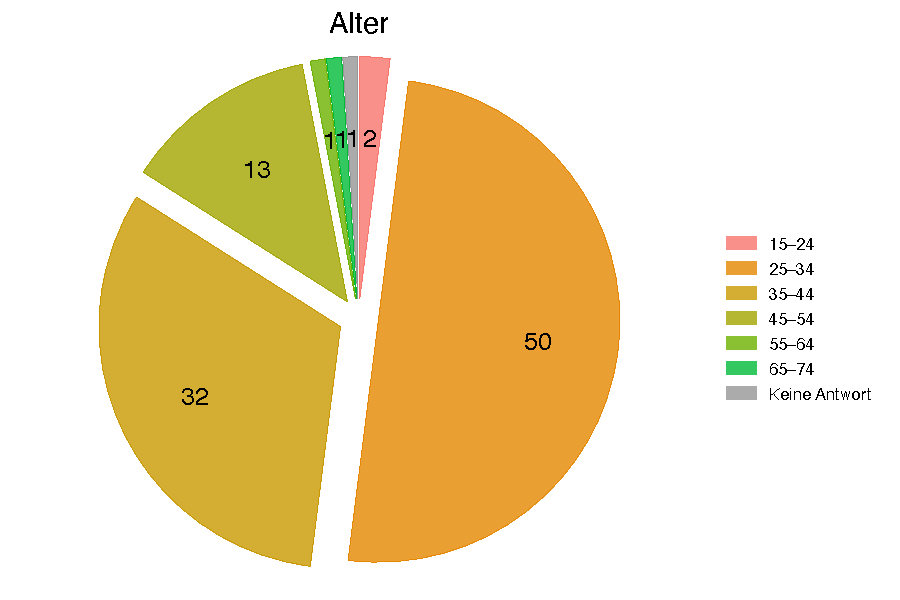
\includegraphics[width=1\textwidth]{alter.pdf}
   \caption{Antworten auf die Aufforderung \enquote{Bitte geben Sie an, in welcher Altersgruppe Sie sich befinden.} (Einfachauswahl)}
   \label{fig:alter}
\end{figure}

Die Geschlechterverteilung (siehe \autoref{fig:gender}) entspricht in etwa unseren Erwartungen; der überwiegende Teil der Teilnehmer:innen (fast genau zwei Drittel) beschreibt sich als \enquote{männlich}, etwas über $20\,\%$ als weiblich, etwa $6\,\%$ als nichtbinär.
Die $4\,\%$ anderen Antworten sind auch im weitesten als im Umfeld queerer Identitäten einzuordnen, konkret waren diese nämlich \enquote{questioning\,/\,demimännlich}, \enquote{männlich\,/\,demigender}, \enquote{divers she-they} -- und einmal schlicht \enquote{nein}, was potenziell als agender interpretiert werden könnte.

\begin{figure}[t]
   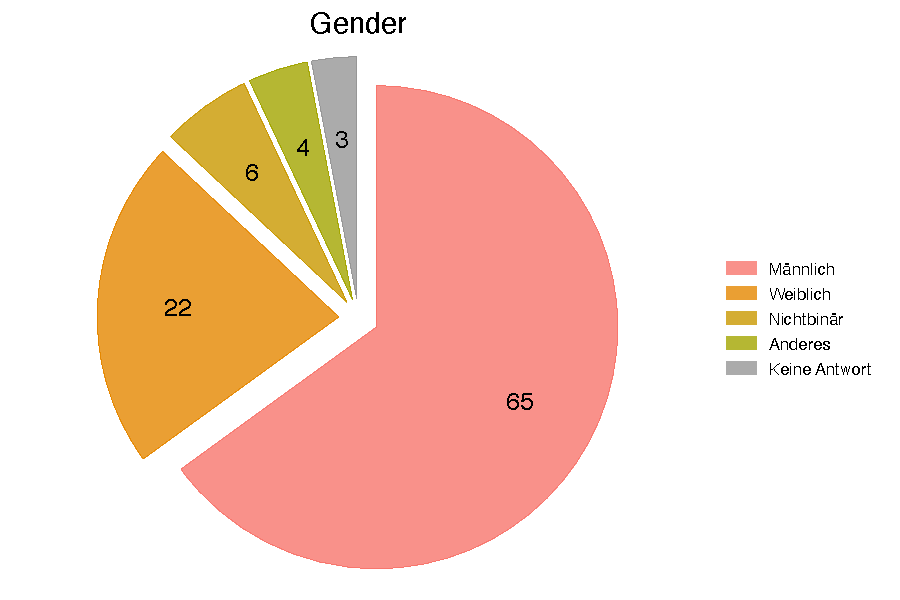
\includegraphics[width=1\textwidth]{gender.pdf}
   \caption{Antworten auf die Aufforderung \enquote{Bitte geben Sie Ihr Geschlecht an.} (Freitextfeld)}
   \label{fig:gender}
\end{figure}

Die Teilnehmer:innen repräsentieren damit bzgl. Alter und Geschlecht das gängige Bild von Game-Studies-Forscher:innen,\footnote{Bei der Auswertung der Geschlechterverteilung der Autor:innen der Zeitschrift \textit{PAIDIA -- Zeitschrift für Computerspielforschung} ergab sich von $2011$ bis $2021$ ein Verhältnis von $63\,\%$ Männern, $34\,\%$ Frauen und $2\,\%$ nichtbinären Personen. Vergleichend waren es bei der Zeitschrift \textit{Game Studies} im Zeitraum von $2001$ bis $2021$ $73\,\%$ Männer, $26\,\%$ Frauen und $1\,\%$ nichtbinäre Personen (\autocite[vgl.][]{unterhuber_offenes_2021}). Beide Verteilungen sind dabei noch nicht einmal Ausreißer im disziplinären Vergleich (\autocite[vgl.][]{west_role_2013}).} wenngleich die Verteilung innerhalb der Gamer:innen-Community doch deutlich ausgeglichener ist, als gemeinhin angenommen wird.\autocite[Vgl. hierzu etwa][S.~13]{rother_spielraume_2025}
Wenn wir diese Daten mit den Daten der angegebenen Disziplinen vergleichen (oder zumindest annähern), welche den Großteil der Befragten umfassen (Literatur- und Sprachwissenschaften, Medienwissenschaften, Geschichte\,/\,Archäologie), ergibt sich wiederum ein etwas anderer Eindruck:
Gerade die Literatur- und Sprachwissenschaften besitzen einen Frauenanteil\footnote{Unsere Vergleichsdaten der Statistik Austria bieten leider nur die binärgeschlechtlichen Optionen männlich\,/\,weiblich an, weswegen wir hier nur von Frauen- und Männeranteilen sprechen können.} von ca. $75\,\%$.\footnote{So ergeben die Daten der Statistik Austria folgendes Bild: Deutsche Philologie (BA): $79,0\,\%$, Deutsche Philologie (MA): $81,2\,\%$, Unterrichtsfach Deutsch (BA): $75,6\,\%$, Unterrichtsfach Deutsch (MA): $78,1\,\%$; Anglistik\,/\,Amerikanistik (BA): $79,9\,\%$, Anglistik\,/\,Amerikanistik (MA): $76,9\,\%$, Unterrichtsfach Englisch (BA): $68,1\,\%$, Unterrichtsfach Englisch (MA): $75,9\,\%$ (\autocite[vgl.][]{statistik_austria_studierende_2025}).}
Ähnliches gilt für medienwissenschaftliche Studiengänge.\footnote{Nach den Daten der Statistik Austria: Medienwissenschaft (MA): $82,6\,\%$ (\autocite[vgl.][]{statistik_austria_studierende_2025}).}
In den historischen Fächern ist das Geschlechterverhältnis hingegen in etwa ausgeglichen (mit Frauenanteilen knapp über oder unter $50\,\%$),\footnote{So zum Beispiel Geschichte (BA): $46,6\,\%$, Geschichte (MA): $53,3\,\%$ (\autocite[vgl.][]{statistik_austria_studierende_2025}).} womit diese auch einen Ausreißer im Vergleich zum Frauenanteil der Geisteswissenschaften allgemein von $69,6\,\%$ darstellen.\autocite[Vgl. wiederum die Daten der][]{statistik_austria_studierende_2025}
Zu beachten ist allerdings, dass sich in den meisten Fächern diese Verhältnisse in den höheren Karrierestufen, teilweise bedrückend deutlich, zu Gunsten der Männer verschieben.\footnote{\autocite[Vgl. z.\,B.][]{blickenstaff_women_2005}, sowie \autocite[][]{innovative_frauen_im_fokus_leaky_2025}.}
Die relativ hohe Beteiligung von Historiker:innen an der Umfrage im Zusammenspiel mit den vertretenen Karrierestufen unter den Teilnehmer:innen erklärt aber aus unserer Sicht den geringen Frauenanteil bei weitem noch nicht.
Wenn ein Großteil der Teilnehmer:innen eigentlich aus einem Fächerspektrum stammt, dessen Frauenanteil im Schnitt deutlich höher als der unserer Teilnehmer:innen ist, muss es weitere Gründe dafür geben.
Sicherlich trägt dazu auch das Image eines männlich codierten Gegenstandes bei, das nicht ganz zu Unrecht auch auf dessen Erforschung übertragen wird.\footnote{\autocite[Vgl.][S.~28]{unterhuber_wer_2024}, sowie \autocite[][S.~214]{vossen_cultural_2018}.}
Es mag aber darüber hinaus auch weitere strukturelle Gründe dafür geben, etwa dass wir bestimmte Gruppen nur unzureichend erreicht haben (persönliche Netzwerk-Effekte; dass alle drei Organisatoren der Studie Männer sind; dass Theoriefragen oft ebenfalls als Männerdomäne begriffen werden; systemischer Ausschluss von Frauen aus wissenschaftlichen Debatten; um nur ein paar spekulative mögliche Ursachen zu nennen).

Bezüglich der Publikationssprache (siehe \autoref{fig:sprache}) ist die überwiegende Antwort (wenig erstaunlich in einer Umfrage unter Forscher:innen in der \textit{deutschsprachigen} Game-Studies-Community) Deutsch.
Angesichts der Tatsache, dass Englisch heutzutage in vielen Feldern die primäre Wissenschaftssprache ist, verwundert aber auch das starke Vorkommen dieser Sprache kaum.
Von den $96$ Personen, die diese Frage beantwortet haben, publizieren $86,5\,\%$ u.\,a. auf Deutsch, $72$ davon (also $75\,\%$ der gegebenen Antworten) vornehmlich auf Deutsch.
Auf Englisch publizieren $59$ Personen (das sind $61,5\,\%$), davon $27$ (also $28,1\,\%$) vornehmlich.\footnote{Wir haben für diese Auswertung jene Personen, die explizit \enquote{Deutsch und Englisch gleichermaßen} (oder ähnliche Formulierungen) geantwortet hatten, sowohl unter \enquote{vornehmlich Deutsch} als auch unter \enquote{vornehmlich Englisch} verbucht.}
Zwei Personen publizieren auf Deutsch, Englisch und Französisch (einmal in der Reihenfolge \enquote{Englisch, Deutsch, Französisch}, einmal \enquote{Französisch, Deutsch, Englisch}).
Erwähnenswert ist vielleicht weiters, dass in etwa die Hälfte der Teilnehmer:innen monolingual publiziert ($50$ Personen, also $52,1\,\%$), die Hälfte in zumindest zwei Sprachen.
Dies mag wiederum mit den jeweiligen Ursprungsdisziplinen zusammenhängen -- so ist die Germanistik aufgrund ihres Gegenstandes (fast) monolingual, ebenso wie Anglistik und Amerikanistik.
Auch in anderen stark und lange in der deutschsprachigen Universitätslandschaft verwurzelten Fächern ist Deutsch für einen gewissen Diskursbereich noch immer die primäre Wissenschaftssprache.

\begin{figure}[t]
   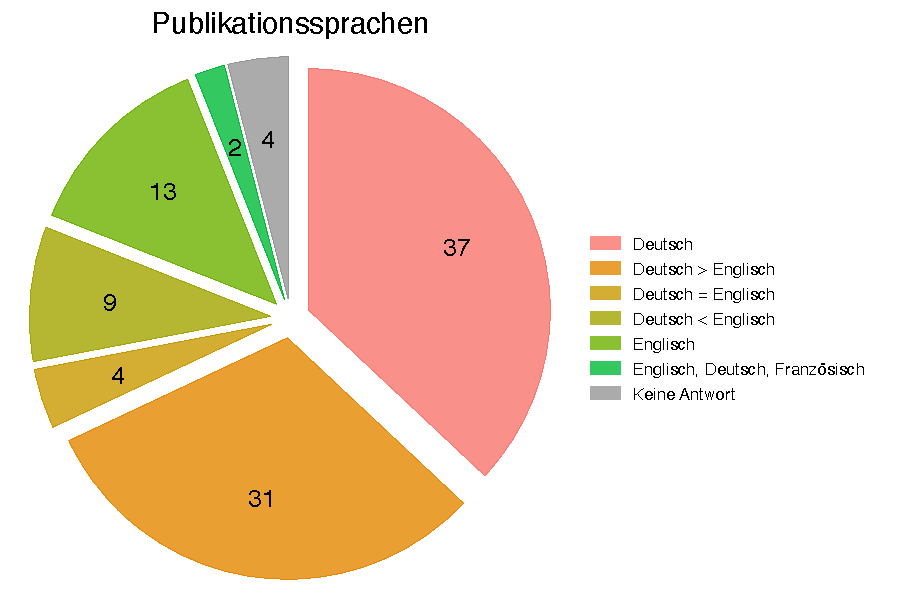
\includegraphics[width=1\textwidth]{sprache.pdf}
   \caption{Antworten auf die Frage \enquote{In welcher Sprache oder welchen Sprachen schreiben Sie Ihre Forschung in den Game Studies primär?} (Freitextfeld)}
   \label{fig:sprache}
\end{figure}

Betreffend einer Zuordnung der Teilnehmer:innen zu Ländern oder Nationalitäten haben wir uns entschieden, nur die Studienorte zu erfragen.
Wegen der Datenkomplexität und relativ geringen Interessanz verzichten wir an dieser Stelle auf eine erschöpfende Auflistung aller Antworten je nach Abschlussart und fassen nur in groben Zügen zusammen:
Das weit überwiegend am häufigsten genannte Land ist Deutschland (über $150$ Nennungen), gefolgt von Österreich ($40$ Nennungen) und der Schweiz ($9$ Nennungen).
Vereinzelt genannt werden weiters Frankreich, Italien, Japan, Malta, Polen, Rumänien, das Vereinigte Königreich und die Vereinigten Staaten (alle jeweils nur ein- oder zweimal).


%%%%%%%%%%%%%%%%%%%%%%%%%
% RESULTATE – VERORTUNG %
%%%%%%%%%%%%%%%%%%%%%%%%%
\subsection{Verortung im Wissenschaftsbetrieb}\label{sec:resultate_verortung}
Es ist uns mit unserer Umfrage (trotz der Tatsache, dass sie als Datenbasis für diesen Beitrag zum Jubiläumssammelband des AKWGDS erstellt wurde) gelungen, Teilnehmer:innen weit über den Arbeitskreis hinaus zu erreichen; die Teilnehmer:innen verteilen sich fast $50:50$ auf Mitglieder und Nichtmitglieder des AKGWDS (siehe \autoref{fig:akgwds}).

\begin{figure}[t]
   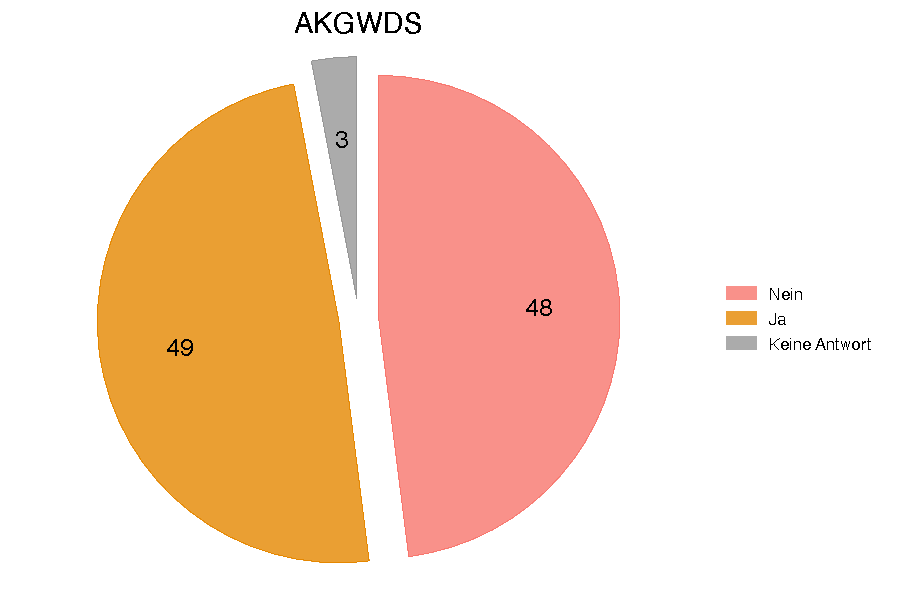
\includegraphics[width=1\textwidth]{akgwds.pdf}
   \caption{Antworten auf die Frage \enquote{Sind Sie Mitglied im AKGWDS?} (Einfachauswahl)}
   \label{fig:akgwds}
\end{figure}

Die Verteilung der akademischen Karrierestufen (siehe \autoref{fig:rolle}) entspricht in etwa unseren Erwartungen; die Rollen \enquote{Student:in} und \enquote{Promovierende:r} bzw. \enquote{wissenschaftliche:r Mitarbeiter:in} sind klar am stärksten vertreten, \enquote{externe:r Forscher:in} und \enquote{Sonstiges} schon merklich seltener, und \enquote{Professor:in} sowie \enquote{Lehrbeauftragte:r\,/\,Do\-zen\-t:in} sind nur sehr geringfügig unter den Umfrage-Teilnehmer:innen vertreten.
Die Rolle \enquote{Juniorprofessor:in}, die wir auch abgefragt hatten, scheint gar nicht auf.
Die Freitextantworten für die dreizehnmal getroffene Rollenauswahl \enquote{Sonstiges} lassen sich wie folgt einordnen:
Es handelt sich überwiegend entweder um überlappende, liminale oder transiente Zustände neben oder zwischen den von uns explizit vorgesehenen Rollen (in fünf Fällen: \enquote{bald promovierend, aber Absolvent:in}, \enquote{ab nächsten Monat wissenschaftliche:r Mitarbeiter:in}, \enquote{promovierend und wissenschaftliche Mitarbeiterin}, \enquote{Ex-Student} sowie \enquote{Masterarbeit gerade beendet}) oder um Rollen im Nahbereich des akademischen Betriebs (ebenfalls in fünf Fällen: \enquote{Lehrer an einer Fachhochschule (Ausland)}, \enquote{Mitarbeiter in Technik und Verwaltung}, \enquote{Verwalterin einer Professur}, \enquote{Postdoc} sowie \enquote{Koordination}).
Die drei anderen Fälle sind tatsächlich \textit{sui generis} (\enquote{Volontär}, \enquote{Museumspädagoge} sowie einmal schlicht keine Angabe).

\begin{figure}[t]
   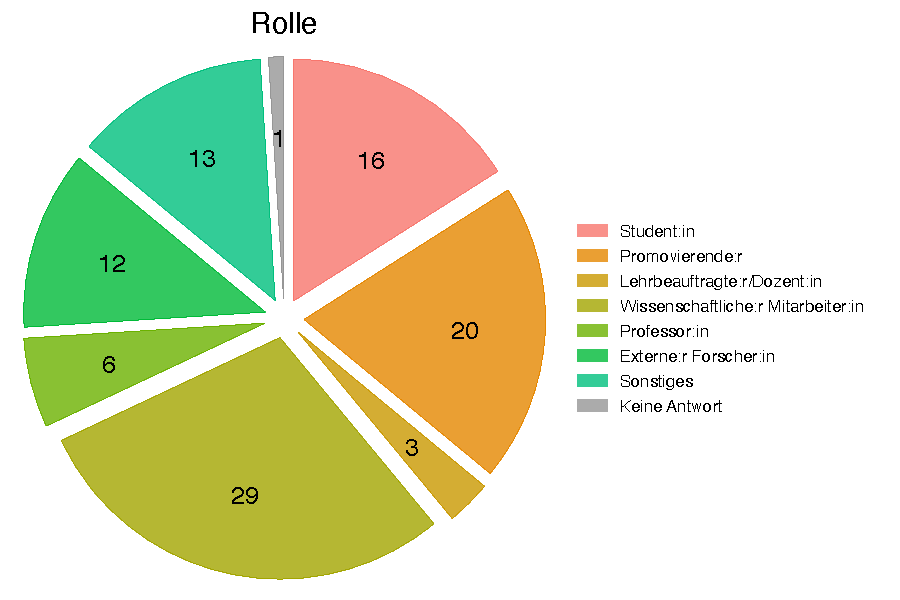
\includegraphics[width=1\textwidth]{rolle.pdf}
   \caption{Antworten auf die Frage \enquote{In welcher akademischen Rolle befinden Sie sich derzeit?} (Einfachauswahl)}
   \label{fig:rolle}
\end{figure}

Wir haben außerdem gefragt, ob die Teilnehmer:innen aktuell oder innerhalb der letzten zwölf Monate in einem wissenschaftlichen Kontext angestellt waren (siehe \autoref{fig:anstellung}).
Die Personen, die derzeit oder in jüngster Vergangenheit keine Position im Wissenschaftsbetrieb hatten ($32$ und damit etwa $32,7\,\%$ derjenigen, die diese Frage beantworteten), verteilen sich recht gleichmäßig auf die Rollen \enquote{Student:in} (zehn Personen), \enquote{Promovierende:r} (sieben Personen) und \enquote{externe:r Forscher:in} (neun Personen).
Der Rest fällt entweder in die Kategorie \enquote{Sonstiges} (fünf Personen, konkret: \enquote{ab nächsten Monat wissenschaftliche:r Mitarbeiter:in}, \enquote{Koordination}, \enquote{Postdoc}, \enquote{Volontär} sowie einmal ohne weitere Spezifizierung) oder, in einem Sonderfall, in die Rolle \enquote{Lehrbeauftragte:r\,/\,Dozent:in}.
Bemerkenswert hieran ist vielleicht noch, dass demnach ein guter Teil der Studierenden, der Großteil der Promovierenden und selbst ein gewisser Anteil der externen Forscher:innen (aktuell oder zumindest in jüngerer Vergangenheit) über irgendeine Form von Anstellungsverhältnis im Wissenschaftsbetrieb verankert waren.
Dies überrascht insofern, als es in den Geisteswissenschaften alles andere als selbstverständlich ist, auf einer bezahlten Stelle zu promovieren (insbesondere im Vergleich zu technischen oder naturwissenschaftlichen Fächern).\footnote{So weist das deutsche Statistische Bundesamt für das Jahr $2024$ unter Promovierenden in den Geisteswissenschaften einen Anteil von Promovierenden \enquote{mit Beschäftigungsverhältnis an der Hochschule der Promotion} von $20,6\,\%$ aus, für Mathematik\,/\,Naturwissenschaften oder Ingenieurwissenschaften hingegen Anteile von $43,1\,\%$ bzw. $44,8\,\%$ (\autocite[vgl.][]{statistisches_bundesamt_tabelle_2025}).}
Ein Teil der Diskrepanz mag darin liegen, dass wir in unserer Umfrage deutlich allgemeiner nach Anstellung \enquote{in einem wissenschaftlichen Kontext} fragen, was auch andere Optionen als bezahlte Dissertationsstellen einschließt.
Andererseits wäre es auch denkbar, dass unsere Umfrage aus verschiedenen Gründen (Netzwerkeffekte etc.) primär jene erreicht hat, die stärker (eben auch über Anstellungsverhältnisse) im wissenschaftlichen Betrieb verankert sind.

\begin{figure}[t]
   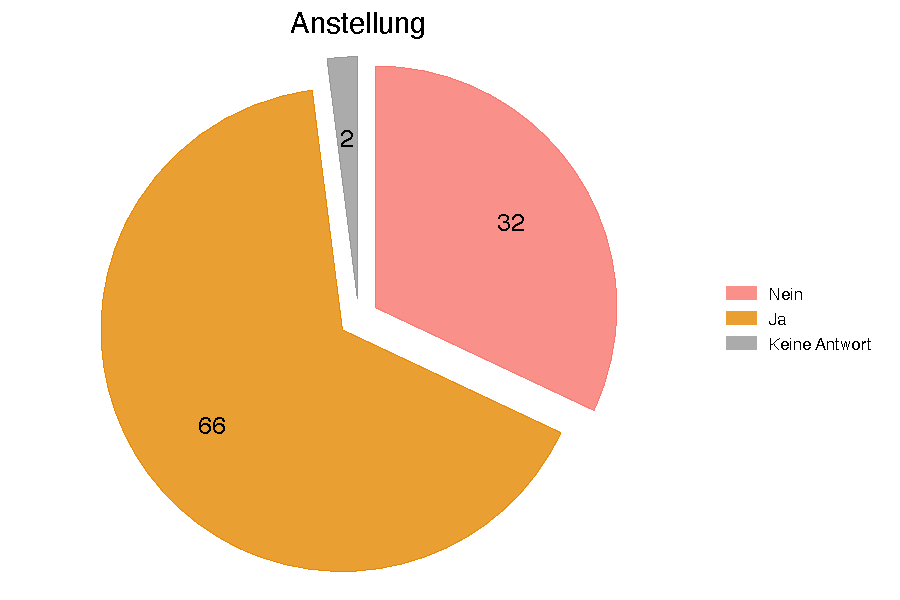
\includegraphics[width=1\textwidth]{anstellung.pdf}
   \caption{Antworten auf die Frage \enquote{Sind Sie aktuell oder waren Sie innerhalb der letzten zwölf Monate in einem wissenschaftlichen Kontext angestellt?} (Einfachauswahl)}
   \label{fig:anstellung}
\end{figure}

All diejenigen Teilnehmer:innen, die auf die obige Frage (\enquote{Sind Sie aktuell oder waren Sie innerhalb der letzten zwölf Monate in einem wissenschaftlichen Kontext angestellt?}) mit \enquote{Ja} geantwortet haben, wurden von uns anschließend anzugeben gebeten, wie sich ihre Aufgaben ungefähr prozentual auf die Bereiche \enquote{Forschung}, \enquote{Lehre} und \enquote{Administratives} aufteilen.
Hierzu konnten sie ganzzahlige Werte zwischen $0$ und $100$ für jede der drei Optionen eingeben, wobei die Summe am Ende $100$ ergeben musste.
In den Antworten (siehe \autoref{fig:aufteilung}) zeigt sich, dass Forschung den breitesten Wertebereich und den höchsten Median ($\text{Median} = 40$, $\text{Mittelwert} = 44,098$) aufweist; Lehre ist im Median etwas niedriger ($\text{Median} = 30$, $\text{Mittelwert} = 34,554$), aber auch stark gestreut.
Administratives liegt hingegen im Median am niedrigsten ($\text{Median} = 20$, $\text{Mittelwert} = 30,859$) und weist die geringste Streuung auf, wobei einige wenige Teilnehmer:innen extrem hohe Werte angegeben haben, was sich bei einzelnen Teilnehmer:innen aus ihrer explizit genannten beruflichen Tätigkeit erklären lässt (konkret \enquote{Mitarbeiter in Technik und Verwaltung} sowie \enquote{Museumspädagoge}).
Diese Werte entsprechen in etwa den durchschnittlichen Werten des Wissenschaftsbarometers $2023$ für Postdocs,\autocite[Vgl.][S.~14--15]{fabian_barometer_2024} auch wenn dieses eine granularere Aufteilung verwendet.
Im Vergleich sticht ins Auge, dass in unseren Ergebnissen der Verwaltungsanteil merklich höher zu sein scheint; dies mag allerdings auch an der weniger detaillierten Aufschlüsselung und dementsprechend am Fehlen laut Wissenschaftsbarometer durchaus relevanter Bereiche wie \enquote{Drittmittelakquise} und \enquote{Begutachtung} liegen, die je nach Interpretation der Teilnehmer:innen mehr als Forschungs- oder mehr als administrative Tätigkeit verstanden werden könnten.

\begin{figure}[t]
   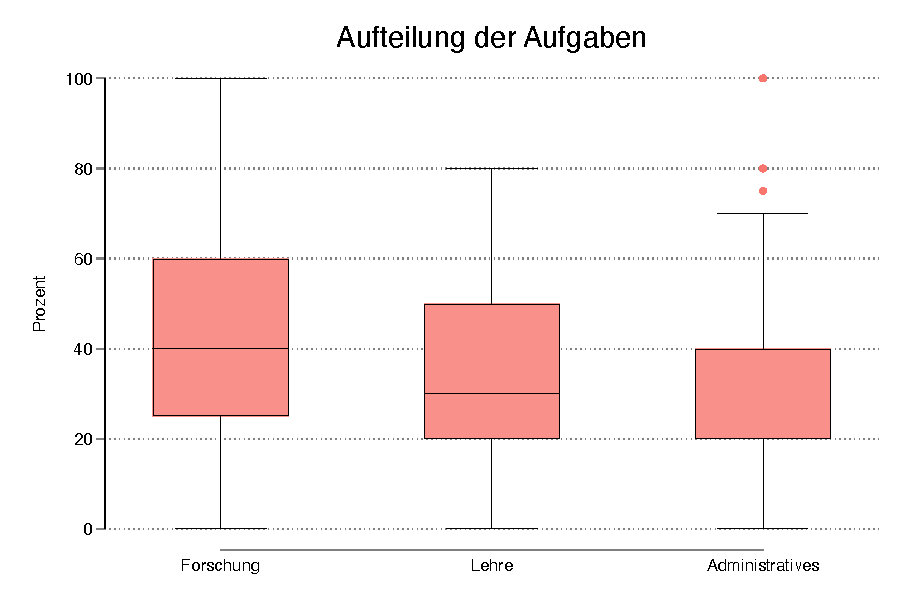
\includegraphics[width=1\textwidth]{aufteilung.pdf}
   \caption{Antworten auf die Aufforderung \enquote{Geben Sie bitte an, wie sich Ihre Aufgaben ungefähr prozentual auf folgende Bereiche aufteilen (bzw. zuletzt aufgeteilt haben).} (numerische Eingabe)}
   \label{fig:aufteilung}
\end{figure}

Die gleichen Teilnehmer:innen wurden anschließend nach der Befristung der eigenen Position gefragt (siehe \autoref{fig:befristung}).
An ihren Antworten zeigen sich die im deutschsprachigen Raum üblichen Probleme mit Prekarität im Wissenschaftsbetrieb; die überwiegende Mehrheit der Personen, die aktuell beruflich eine wissenschaftliche Position innehaben, sind nur befristet angestellt ($48$ von $66$, also $72,7\,\%$).
Die fünf Personen ($9,1\,\%$) mit einer Form von Sonderkündigungsschutz sind in drei Fällen Professor:innen, die anderen beiden sind Spezialfälle (einmal laut Freitextantwort zur Rollenauswahl \enquote{Sonstiges} \enquote{Lehrer an einer Fachhochschule (Ausland)}, einmal externe:r Forscher:in).
Dreizehn Personen ($19,7\,\%$) sind im herkömmlichen Sinne unbefristet angestellt, wobei der überwiegende Anteil davon ($9$ von $13$, also $69,2\,\%$) als wissenschaftliche Mitarbeiter:innen angestellt sind; zwei sind Professor:innen (allerdings eben ohne Sonderkündigungsschutz), einer fällt als \enquote{Mitarbeiter in Technik und Verwaltung} unter die Rolle \enquote{Sonstiges} -- und in einem Fall koinzidiert eine unbefristete Anstellung mit der Rollenauswahl \enquote{Student:in}, was ein Versehen oder schlicht ein etwas atypischer Sonderfall sein mag.

\begin{figure}[t]
   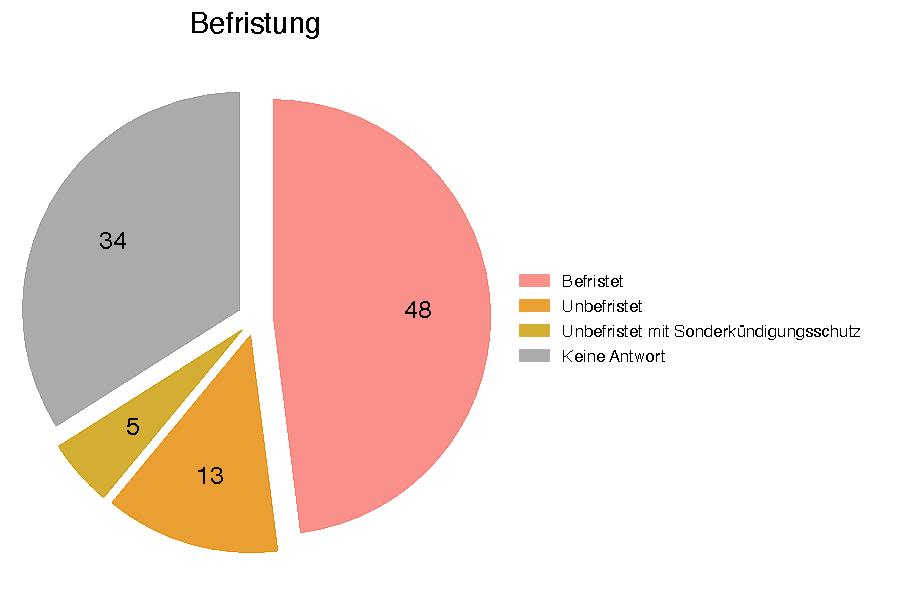
\includegraphics[width=1\textwidth]{befristung.pdf}
   \caption{Antworten auf die Frage \enquote{Sind Sie derzeit befristet oder unbefristet angestellt?} (Einfachauswahl)}
   \label{fig:befristung}
\end{figure}


%%%%%%%%%%%%%%%%%%%%%%%%%%%%%%
% RESULTATE – STUDIENFAECHER %
%%%%%%%%%%%%%%%%%%%%%%%%%%%%%%
\subsection{Studienfächer}\label{sec:resultate_studienfaecher}
Wir verwenden die Österreichische Systematik der Wissenschaftszweige der Statistik Austria.\autocite[Vgl.][]{statistik_austria_schlagwortverzeichnis_2023}
Der weit überwiegende Teil der Freitextantworten ließ sich nach dieser Systematik ohne Entscheidungsbedarf unsererseits eindeutig zuordnen (siehe \autoref{tab:studienfaecher} in Appendix B); bei einigen wenigen Fällen haben wir folgende Anpassungen bzw. erforderlichen ergänzenden Zuweisungsentscheidungen vorgenommen:

\begin{itemize}
   \item \enquote{Digital Humanities} haben wir wegen der großen Relevanz und schweren Zuordenbarkeit als eigenen Studienbereich verzeichnet.\footnote{Siehe zu Wechselwirkungen, Parallelen und Querbezügen zwischen Digital Humanities und Game Studies auch den Text von Brandenburg, Demleitner, Färberböck, Klausner und Nieser in diesem Band.}
   \item \enquote{Digital History}, \enquote{Kulturgeschichte} sowie \enquote{Zeitgeschichte und Medien} haben wir \enquote{Geschichte, Archäologie} zugeordnet.
   \item \enquote{Künstliche Intelligenz} haben wir unter \enquote{Informatik} verbucht.
   \item \enquote{Kulturwissenschaften} ist bei Statistik Austria nicht als eigenes Fach eingetragen, aber wohl ohne großen Argumentationsbedarf dem Bereich \enquote{Kulturwissenschaften} zuzuschreiben.\footnote{Auch wenn hier vielleicht die Kulturwissenschaft, die Kulturwissenschaften und die Kulturwissenschaft(en) unterschiedlicher Meinung sein könnten.}
   \item \enquote{Dramaturgie}, \enquote{Game Development and Research}, \enquote{Game Studies} sowie \enquote{World Arts and Music} haben wir \enquote{Kunstwissenschaften} zugewiesen.
   \item \enquote{Bibliotheksmanagement}, \enquote{Film- und Medienkulturforschung}, \enquote{Filmwissenschaft}, \enquote{Medien und kulturelle Praxis}, \enquote{Medienkultur}, \enquote{Medienkulturwissen\-schaft}, \enquote{Thea\-ter- und Medienwissenschaften} sowie \enquote{Theater-, Film- und Medienwissenschaft} haben wir alle im Bereich \enquote{Medien- und Kommunikationswissenschaften} eingeordnet.
   \item \enquote{Politik–Wirtschaft} haben wir \enquote{Politikwissenschaften} zugewiesen.
   \item \enquote{Gesellschaftswissenschaften} haben wir als zu \enquote{Soziologie} gehörig verstanden.
   \item \enquote{Buchwissenschaft}, \enquote{Kulturpoetik der Literatur und Medien}, \enquote{Literatur und Medien} sowie \enquote{Literatur-, Sprach-, Kulturwissenschaften} haben wir alle unter \enquote{Sprach- und Literaturwissenschaften} subsumiert.
   \item \enquote{Arbeitsgestaltung und HR-Management} sowie \enquote{Wirtschaft} haben wir schließlich beide unter \enquote{Wirtschaftswissenschaften} eingetragen.
\end{itemize}

Auf der Grundlage von:
\enquote{Welche akademischen Abschlüsse haben Sie bisher erworben?} (siehe \autoref{tab:studienbereiche} in Appendix B für die zugrundeliegenden Zahlen) in Zusammenspiel mit dem Freitextfeld zur Beschreibung des Fachs ergibt sich unter diesen Voraussetzungen demnach das folgende Bild (siehe \autoref{fig:bereiche}).

\begin{figure}[t]
   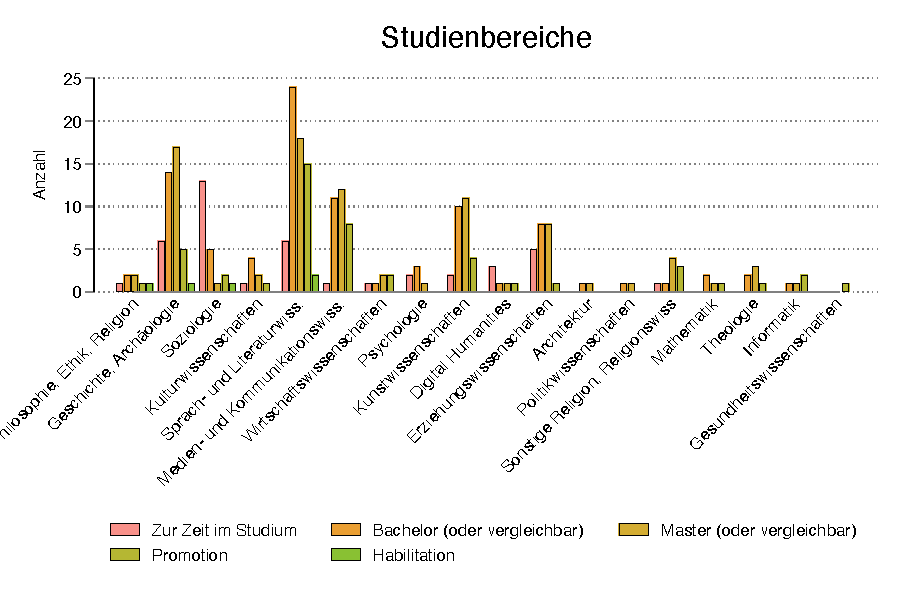
\includegraphics[width=1\textwidth]{bereiche.pdf}
   \caption{Strukturierte Gruppierung der Antworten auf die Frage \enquote{Welche akademischen Abschlüsse haben Sie bisher erworben?} (Freitextfeld)}
   \label{fig:bereiche}
\end{figure}

Auffällig ist hieran insbesondere die generelle Häufung der Antworten bei (in etwa absteigend in dieser Reihenfolge) \enquote{Sprach- und Literaturwissenschaften}, \enquote{Geschichte, Archäologie}, \enquote{Medien- und Kommunikationswissenschaften}, \enquote{Kunstwissenschaften} sowie \enquote{Erziehungswissenschaften}.
Die Befassung mit Game Studies erfolgt also (neben dem teilweise auch aus der Historie des AKGWDS als ursprünglich \enquote{Arbeitskreis Geschichtswissenschaft und Digitale Spiele} erklärbaren Cluster in Geschichte\,/\,Archäologie, primär in literatur- und medienwissenschaftlichen Studiengängen, die ja auch historisch oft miteinander in Beziehung stehen.
Dies mag auch insofern nicht verwundern, da insbesondere Germanistik-Institute im deutschsprachigen Raum genauso wie Englisch-Institute im anglophonen Raum als \enquote*{große Fächer} gelten können, also Fächer, die (zumindest früher) eine große Anzahl Studierender und damit auch Lehrender besaßen (tw. auch wegen der engen Verknüpfung mit entsprechenden Lehramtsstudien), was sich auf die Möglichkeit neue Felder, Zugänge etc. auszuprobieren und zu entwickeln auswirkte:\footnote{Die unter anderem von Albrecht Koschorke formulierte These, die Germanistik befände sich \enquote{auf dem Weg zum kleinen Fach}, verkennt, dass die Germanistik schon seit langem Inkubator für neue Forschungsgegenstände und -richtungen war und diese Funktion eben eine Kernkompetenz des Faches darstellt -- während die von Koschorke ins Feld geführte \enquote{legitimatorische Grundlage [$\ldots$] als Nationalphilologie und damit als nationalkulturelles Unternehmen} (fast schon klischeehaft für einen Deutschen) übersieht, dass Germanistik immer schon mindestens drei Nationalliteraturen unter ihrem Dach vereinte (oder zumindest vereinen sollte) (\autocite[vgl.][S.~590]{koschorke_germanistik_2015}).}
Wenn es ausreichend Personal gibt, das bereits die kanonisierte und grundständige Lehre abdeckt, gibt es dementsprechend mehr Spielraum für Experimente und neuartige Zugänge.\footnote{Vgl. zur Entwicklung der Hamburger Medienwissenschaft in und aus der Germanistik \autocite[][S.~35–56]{hickethier_binnendifferenzierung_2000}.}
Darüber hinaus gibt es aber auch bereits zwischen Literatur- und Medienwissenschaft eine Nähe der Gegenstände, die historisch auch immer näher zusammenrückten (befördert durch das gemeinsame Interesse an Fragen der Ästhetik etc.).
Ansonsten sticht noch ins Auge, dass es eine große Anzahl von Studierenden bei \enquote{Soziologie} gibt -- wir wissen keinen offensichtlichen Grund für diesen Ausreißer, können uns aber vorstellen, dass unsere Umfrage potenziell dort in Studierenden-Kreisen geteilt wurde.


%%%%%%%%%%%%%%%%%%%%%%%%%%
% RESULTATE – PROVENIENZ %
%%%%%%%%%%%%%%%%%%%%%%%%%%
\subsection{Provenienz der Methodenkenntnisse}\label{sec:resultate_provenienz}
Unsere Teilnehmer:innen wurden von uns gefragt, in welchen Kontexten sie diejenigen methodischen Ansätze erlernt haben, die sie in ihrer Forschung außerhalb der Game Studies verwenden, und in welchen Kontexten sie diejenigen methodischen Ansätze erlernt haben, die sie in ihrer Forschung innerhalb der Game Studies verwenden.
In beiden Fällen konnten beliebig viele Antwortoptionen gewählt werden, wobei wir als mögliche Kontexte \enquote{im Rahmen des Bachelorstudiums (oder eines vergleichbaren Studiums)}, \enquote{im Rahmen des Masterstudiums (oder eines vergleichbaren Studiums)}, \enquote{im Rahmen des Promotionsstudiums}, \enquote{durch Selbststudium} und \enquote{Sonstiges} zur Verfügung gestellt haben.

Bezüglich der Forschung \textit{außerhalb} der Game Studies (siehe \autoref{fig:whkontext}) scheinen die relevanten Methoden vorrangig durch das Bachelor- und Masterstudium sowie durch autodidaktische Initiative erworben worden zu sein.
Alle drei Optionen sind rund $50$-mal vertreten.
Nur etwa halb so häufig, nämlich $27$-mal, wird angegeben, dass diese Methoden während der Promotionsphase erworben wurden.
Die neun Nennungen unter \enquote{Sonstiges} umfassen unter anderem einmal die Habilitation sowie mehrfach die Zeit im Beruf, wobei zumindest in zwei Fällen deutlich wird, dass dabei die berufliche Praxis als Wissenschaftler:in gemeint ist (durch die Freitextantworten \enquote{bei der Arbeit als Wissenschaftler} sowie \enquote{Forschung}).

\begin{figure}[t]
   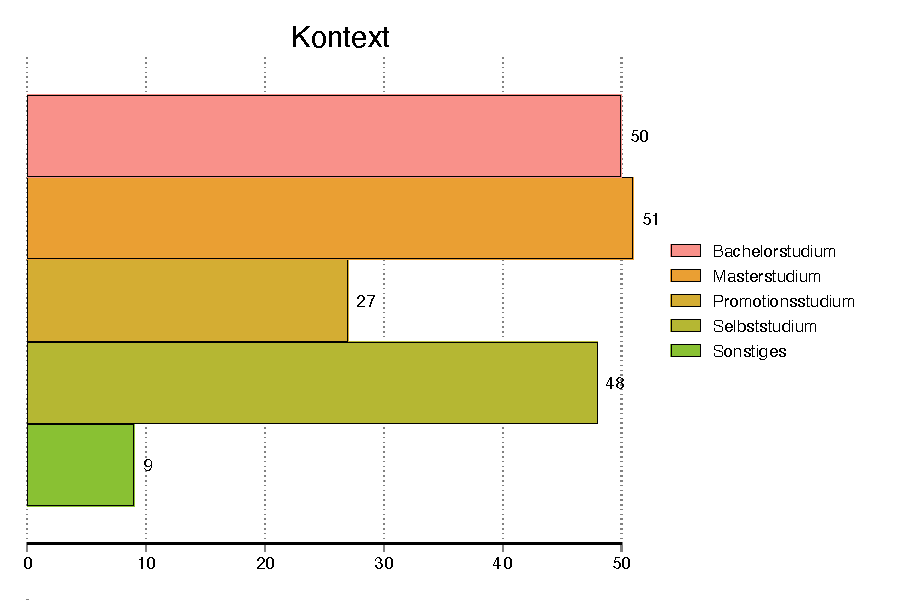
\includegraphics[width=1\textwidth]{whkontext.pdf}
   \caption{Antworten auf die Frage \enquote{In welchem Kontext haben Sie die methodischen Ansätze, die Sie in Ihrer Forschung außerhalb der Game Studies verwenden, erlernt?} (Mehrfachauswahl)}
   \label{fig:whkontext}
\end{figure}

In Hinsicht auf die Forschung \textit{innerhalb} der Game Studies (siehe \autoref{fig:gskontext}) dominieren ebenfalls Bachelor-, Master- und Selbststudium.
Bachelor- und Selbststudium sind erneut rund $50$-mal vertreten, das Masterstudium rund $60$-mal.
Die Zahl derjenigen, die die Promotionszeit als Kontext angegeben haben, ist mit $40$ Nennungen hingegen merklich höher als in der Forschung außerhalb der Game Studies.
Die acht Einträge unter \enquote{Sonstiges} umfassen hier erneut einmal die Habilitation sowie mehrfach die Zeit im Beruf, wobei neben der beruflichen Praxis als Wissenschaftler:in auch diejenige als Journalist:in explizit Erwähnung findet.

\begin{figure}[t]
   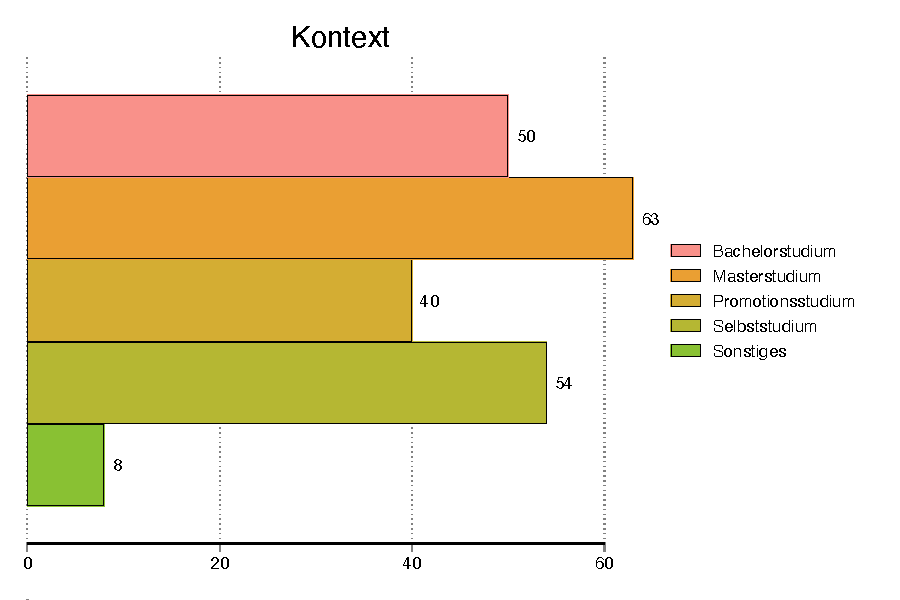
\includegraphics[width=1\textwidth]{gskontext.pdf}
   \caption{Antworten auf die Frage \enquote{In welchem Kontext haben Sie diese methodischen Ansätze [Ihrer Forschung in den Game Studies] erlernt?} (Mehrfachauswahl)}
   \label{fig:gskontext}
\end{figure}

Insgesamt zeigt sich damit einerseits, dass der relevante Kontext -- sowohl zur Forschung \textit{innerhalb} als auch \textit{außerhalb} der Game Studies -- nicht uniform ist; keine der Optionen repräsentiert eine überwältigende Mehrheit unserer Teilnehmer:innen.
Stattdessen mäandern Bachelor-, Master- und Selbststudium mit den häufigsten Nennungen um etwa $50$ (in einem Fall bis um etwa $60$) herum.
Andererseits wird auch deutlich, dass der Erwerb relevanter Methodenkenntnisse für einige bereits im Bachelorstudium beginnt, sich für ebenso viele während des Masters abspielt, für viele aber auch in der Promotionszeit (und in einem Fall sogar in der Zeit der Habilitation) stattfindet.
Rund $30$ beziehungsweise $40$ Nennungen weisen außerdem auf eine deutliche Bereitschaft zum autodidaktischen Erwerb von Methodenkenntnissen hin.
Die häufige Anführung des Selbststudiums ist, gerade weil ein Großteil der Teilnehmer:innen aus den Geisteswissenschaften stammt (vgl. \autoref{sec:resultate_studienfaecher}), wo die selbständige Aneignung von Wissen eigentlich strukturell zum Studium gehört, auch nicht weiter verwunderlich.
(Gleichzeitig kann man es durchaus kritisch sehen, dass in vielen Fächern offenbar selbst methodische und theoretische Grundlagenkenntnisse gar nicht oder zumindest nicht ausreichend im Rahmen von Lehrveranstaltungen vermittelt werden.)

Im direkten Vergleich der beiden Antwortverteilungen sticht zuletzt noch ins Auge, dass beim Aneignungszeitpunkt der methodischen Kenntnisse für die Forschung innerhalb der Game Studies eine leichte (statistisch nicht signifikante; Wald $\chi^{2}(4) = 1,44$, $p = 0,838$) Verschiebung nach hinten im akademischen Verlauf vorliegt, insofern mit $63$ vs. $51$ Nennungen des Masterstudiums bzw. $40$ statt $27$ Nennungen des Doktoratsstudiums ein merklicher Anstieg zu erkennen ist, wohingegen das Bachelorstudium bei beiden Fragen gleichermaßen $50$-mal als Antwort gewählt wurde.
Dies spricht dafür, dass Methoden und Theorien zur Erforschung von Spielen nicht so sehr Teil der grundständigen Lehre sind wie andere Methoden.
Wir vermuten, dass der Grundstock erlernter Zugänge, der einerseits die fachliche Zurichtung mit sich bringt, aber gleichzeitig auch medienunabhängig angewandt werden kann, in späteren Karrierephasen und der damit einhergehenden Spezialisierung um spezifische Inhalte der Game Studies ergänzt wird.


%%%%%%%%%%%%%%%%%%%%%%%%%%%%%%%%%%%
% RESULTATE – SELBSTEINSCHAETZUNG %
%%%%%%%%%%%%%%%%%%%%%%%%%%%%%%%%%%%
\subsection{Selbsteinschätzung des methodischen Vorgehens}\label{sec:resultate_selbsteinschätzung}
In vier Fragen haben wir unsere Teilnehmer:innen weiters gebeten, ihr methodisches Vorgehen hinsichtlich eigener Vertrautheit, Orthodoxie, Etabliertheit sowie Gebräuchlichkeit einzuschätzen.

Auf die Frage \enquote{Wie gut sind Sie mit dem von Ihnen am häufigsten verwendeten methodischen Ansatz, den Sie derzeit in Ihrer Forschung in den Game Studies verwenden, vertraut?} (siehe \autoref{fig:vertrautheit}) antworten die meisten Teilnehmer:innen mit \enquote{eher vertraut} ($40$ Nennungen) oder \enquote{sehr vertraut} ($38$ Nennungen).
Lediglich $20$ Personen geben an, mit ihnen \enquote{eher unvertraut} ($9$ Nennungen) oder \enquote{sehr unvertraut} ($11$ Nennungen) zu sein.
Ein genauerer Blick in die Daten (siehe \autoref{tab:rollevertrautheit} in Appendix B) zeigt außerdem, dass es sich hierbei nicht (nur) um Teilnehmer:innen an ihrem Karrierebeginn handelt, sondern dass auch alle anderen Karrierestufen (siehe \autoref{sec:resultate_verortung}) vertreten sind ($\chi^{2}(18, 97) = 12,891$, $p = 0,798$).

\begin{figure}[t]
   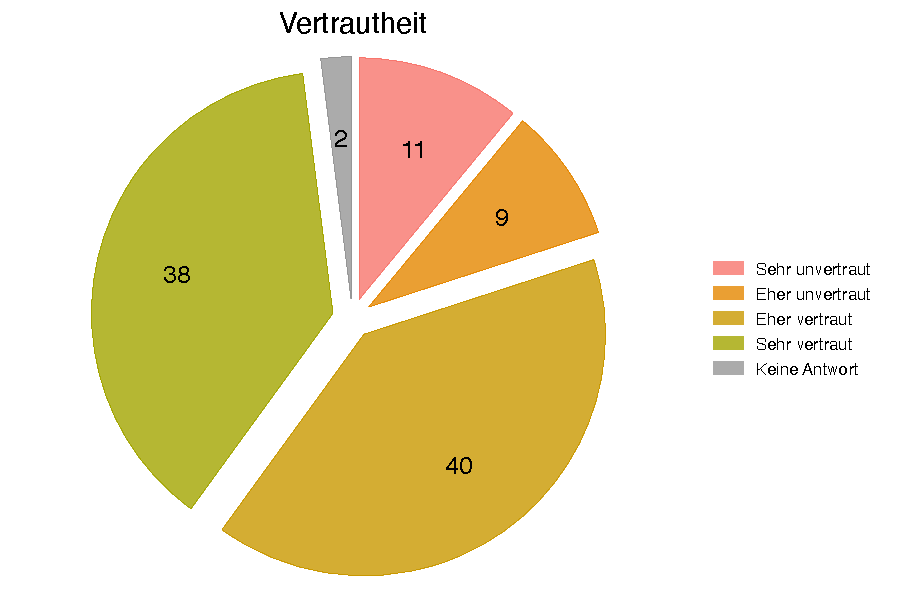
\includegraphics[width=1\textwidth]{vertrautheit.pdf}
   \caption{Antworten auf die Frage \enquote{Wie gut sind Sie mit dem von Ihnen am häufigsten verwendeten methodischen Ansatz, den Sie derzeit in Ihrer Forschung in den Game Studies verwenden, vertraut?} (Einfachauswahl)}
   \label{fig:vertrautheit}
\end{figure}

Auf die Frage \enquote{Wie etabliert oder aktuell schätzen Sie den von Ihnen am häufigsten verwendeten methodischen Ansatz, den Sie derzeit in Ihrer Forschung in den Game Studies verwenden, innerhalb des disziplinären Kontexts ein, in dem Sie ihn ursprünglich erlernt oder kennengelernt haben?} (siehe \autoref{fig:etabliertheit}) antworten etwas mehr als zwei Drittel, dass der Ansatz dort \enquote{etabliert} ($51$ Nennungen) oder \enquote{quasi Standard} ($19$ Nennungen) ist.
Nur ein Zehntel gibt an, dass ihr Ansatz dort \enquote{überhaupt nicht etabliert} ist ($10$ Nennungen).

\begin{figure}[t]
   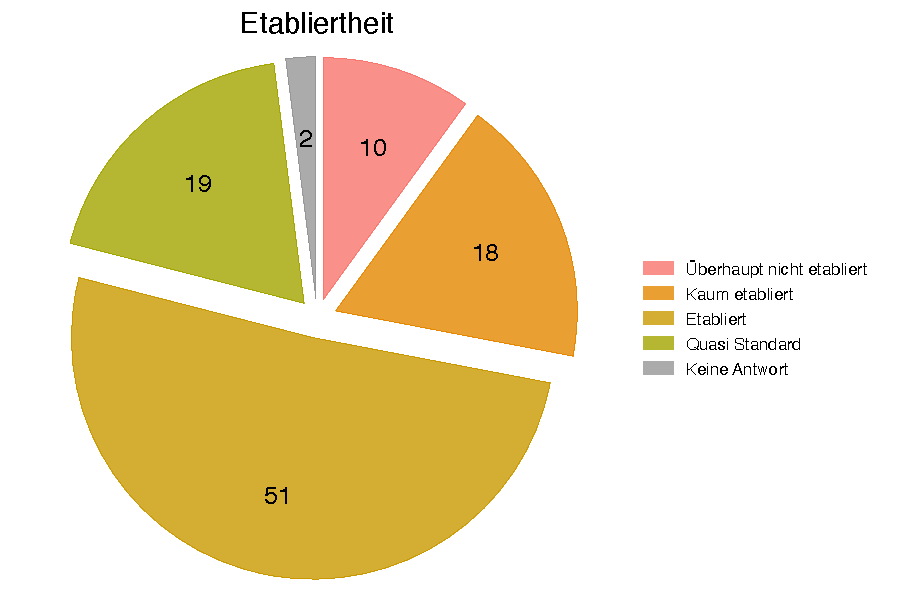
\includegraphics[width=1\textwidth]{etabliertheit.pdf}
   \caption{Antworten auf die Frage \enquote{Wie etabliert oder aktuell schätzen Sie den von Ihnen am häufigsten verwendeten methodischen Ansatz, den Sie derzeit in Ihrer Forschung in den Game Studies verwenden, innerhalb des disziplinären Kontexts ein, in dem Sie ihn ursprünglich erlernt oder kennengelernt haben?} (Einfachauswahl)}
   \label{fig:etabliertheit}
\end{figure}

Auf die Frage \enquote{Wie gebräuchlich schätzen Sie den von Ihnen am häufigsten verwendeten methodischen Ansatz, den Sie derzeit in Ihrer Forschung in den Game Studies verwenden, innerhalb des disziplinären Kontexts ein, in dem Sie ihn ursprünglich erlernt oder kennengelernt haben?} (siehe \autoref{fig:gebraeuchlichkeit}) antwortet ein knappes Drittel unserer Teilnehmer:innen, dass ihr Ansatz dort \enquote{sehr ungewöhnlich} ($8$ Nennungen) oder \enquote{eher ausgefallen} ($21$ Nennungen) ist.
Die Mehrheit geht davon aus, dass ihr Ansatz dort \enquote{gängige Methode} ($41$ Nennungen) oder \enquote{methodischer Standard} ($21$ Nennungen) ist.

\begin{figure}[t]
   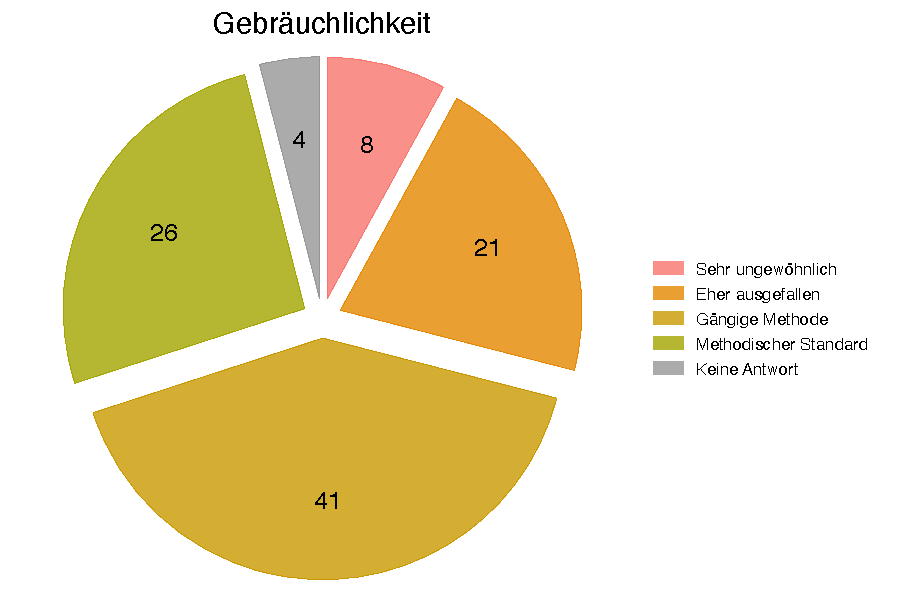
\includegraphics[width=1\textwidth]{gebraeuchlichkeit.pdf}
   \caption{Antworten auf die Frage \enquote{Wie gebräuchlich schätzen Sie den von Ihnen am häufigsten verwendeten methodischen Ansatz, den Sie derzeit in Ihrer Forschung in den Game Studies verwenden, innerhalb des disziplinären Kontexts ein, in dem Sie ihn ursprünglich erlernt oder kennengelernt haben?} (Einfachauswahl)}
   \label{fig:gebraeuchlichkeit}
\end{figure}

Mehr als die Hälfte unserer Teilnehmer:innen antwortet auf die Frage \enquote{Wie schätzen Sie Ihr eigenes methodisches Vorgehen in den Game Studies ein?} (siehe \autoref{fig:orthodoxie}), dass sie es für \enquote{sehr unorthodox bzw. experimentell} ($9$ Nennungen) oder \enquote{eher unorthodox bzw. experimentell} ($52$ Nennungen) halten.
Etwa ein Drittel hält das eigene Vorgehen für \enquote{eher traditionell bzw. disziplinär verankert} ($35$ Nennungen), eine verschwindend geringe Minderheit für \enquote{sehr traditionell bzw. disziplinär verankert} ($3$ Nennungen).

\begin{figure}[t]
   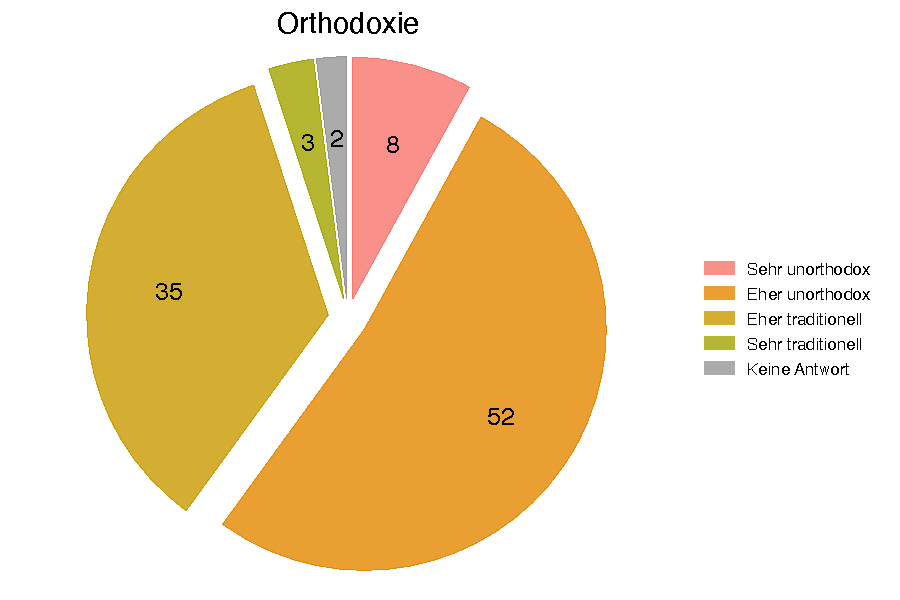
\includegraphics[width=1\textwidth]{orthodoxie.pdf}
   \caption{Antworten auf die Frage \enquote{Wie schätzen Sie Ihr eigenes methodisches Vorgehen in den Game Studies ein?} (Einfachauswahl)}
   \label{fig:orthodoxie}
\end{figure}

Zusammengenommen zeigt sich damit also, dass eine Mehrheit unserer Teilnehmer:in\-nen davon ausgeht, mit dem von ihnen am häufigsten verwendeten methodischen Ansatz, den sie derzeit in ihrer Forschung in den Game Studies verwenden, (sehr) gut vertraut zu sein.
Innerhalb des disziplinären Kontexts, in dem dieser Ansatz ursprünglich erlernt oder kennengelernt wurde, wird er von einer Mehrheit für etabliert beziehungsweise für Standard gehalten, der dort auch entsprechend als gängige Methode oder methodischer Standard aktuell Verwendung findet.
Innerhalb der Game Studies wird dieser von ihnen meistverwendete Ansatz dann allerdings überwiegend als \enquote{eher} oder sogar \enquote{sehr unorthodox} wahrgenommen (wobei insgesamt jedenfalls die gemäßigten Meinungen vorherrschen; nur knapp $10\,\%$ fanden ihr eigenes methodisches Vorgehen in den Game Studies entweder \enquote{sehr traditionell} oder \enquote{sehr unorthodox}).


%%%%%%%%%%%%%%%%%%%%%%%%
% RESULTATE – METHODEN %
%%%%%%%%%%%%%%%%%%%%%%%%
\subsection{Beschreibung der erlernten und verwendeten Methoden}\label{sec:resultate_methoden}
Zuletzt wollen wir uns noch inhaltlich mit den Freitextantworten auf die Fragen nach den innerhalb bzw. außerhalb des Studiums erlernten und in der Game-Studies-Forschung verwendeten Methoden befassen, wobei wir diese Freitextantworten abschließend auch mit den quantitativen Daten aus dem vorangegangenen Abschnitt in Beziehung setzen werden.\footnote{Auf eine graphische Darstellung bzw. numerische Auswertung der Antworten verzichten wir an dieser Stelle bewusst und stellen vielmehr eine qualitative Diskussion der Antworten in den Vordergrund; wir erwarten uns von einer umfassenden quantitativen Aufarbeitung der Freitextantworten (etwa hinsichtlich der explizit genannten Methoden) keinen großen zusätzlichen Erkenntnisgewinn im Vergleich zur bereits in \autoref{sec:resultate_studienfaecher} abgehandelten Verortung der disziplinären Bezüge.}
Mehrere Antworten zur Wahl der eigenen Methoden argumentieren, dass diese eben aus dem erlernten Repertoire stammen und dies damit arbeitsökonomisch oder auch bezogen auf durch die Ursprungsdisziplin beeinflusste Erkenntnisinteressen gewählt würden.
Auch forschungspragmatische Gründe oder die Passgenauigkeit für die eigene Forschungsfrage sowie eine intrinsische Begründung werden mehrfach aufgeführt.
Eine interessante Einzelantwort ist, dass die gewählten Methoden \enquote{in Lehrveranstaltungen} vorgeschrieben worden seien.

Was die explizit genannten Methoden betrifft, die Verwendung finden, zeigt sich ein breites Spektrum an Ansätzen.
Die Auswertung der einzelnen Antworten wird zusätzlich dadurch erschwert, dass ein Teil der Angaben eher auf konkrete methodische und theoretische Zugänge verweist, ein anderer Teil hingegen eher \enquote{Meta-Ausrichtungen} wie \enquote{qualitativ} ($10$-mal), \enquote{interpretativ} ($5$-mal) oder \enquote{quantitativ} ($3$-mal) sowie eher disziplinäre Verortungen wie \enquote{kulturwissenschaftlich} ($5$-mal) anführt.
Wie dem auch sei, bei den konkreter beschriebenen Zugängen gibt es einige Häufungen:
So wird \enquote{Diskursanalyse} $16$-mal (davon $2$-mal geschichtswissenschaftlich, $1$-mal sprachwissenschaftlich, $13$-mal nicht eindeutig zuordenbar), \enquote{Quellenforschung\,/\,-kritik} $12$-mal, \enquote{Interviews} $9$-mal, \enquote{Hermeneutik} $8$-mal, \enquote{Inhaltsanalyse} $8$-mal, \enquote{Rezeptionstheorie\,/\,-ästhetik} $8$-mal, \enquote{(Auto-)Ethnographie} $7$-mal, \enquote{Close Playing} und\,/\,oder \enquote{Close Reading} $6$-mal, \enquote{Narratologie} $6$-mal und \enquote{Oral History} $5$-mal genannt.
Jeweils $4$-mal genannt werden \enquote{Bild-\,/\,Filmanalyse}, \enquote{Distant\,/\,Wide Playing} und\,/\,oder \enquote{Distant\,/\,Wide Reading}, \enquote{Grounded Theory}, \enquote{Medienarchäologie}, \enquote{(Neo-)Phänomenologie} und \enquote{Semiotik}.
Jeweils $3$-mal genannt werden \enquote{Dekonstruktivismus}, \enquote{historisch-kritische Methode}, \enquote{Ideengeschichte}, \enquote{Multimodalität} sowie \enquote{Queer\,/\,Gender Studies}.
(Alle weiteren der insgesamt rund $250$ Einzelnennungen finden nur ein- oder zweimal Erwähnung.)

In diesen Antworten zeigt sich, dass es in den Game Studies zwar sowohl qualitative als auch quantitative Forschung gibt, die qualitativen Ansätze aber deutlich überwiegen.
Weiterhin bewegen sich viele der Ansätze im in den Literatur- und Medienwissenschaften etablierten Theorie- und Methodenkanon; in einigen Fällen handelt es sich bei den häufigeren Antworten auch um genuin geschichtswissenschaftliche Ansätze.
Erwähnenswert ist auch, dass sich nur wenige der genannten Ansätze genuin auf Spiele beziehen -- so wurde etwa \enquote{Game Analysis} nur ein einziges Mal genannt.
Die Vielfalt der aufgeführten Ansätze zeigt zudem, dass auch das deutschsprachige Feld der Game Studies einen klaren, wenn vielleicht auch nicht immer offen diskutierten Methodenpluralismus aufweist, was zeigt:
\enquote{[G]ame studies has inherited not so much the contents of their parental fields but these basic structures and conceptions of what a research field even is}\footnote{\autocite[][S.~236]{unterhuber_parents_2025}; Hervorhebung im Original.}

Die abschließenden Freitextantworten wurden von vielen Teilnehmer:innen für aus unserer Sicht sehr spannende weitergehende Überlegungen genutzt.
Schon die Frage nach Methodik an sich brachte gewisse Probleme in der Beantwortung mit sich.
Viele geisteswissenschaftliche Fächer formulieren nur sehr uneindeutig, was eine Methode überhaupt ist und was als Methode bezeichnet werden kann.
Hier mag auch die allgemeine Vorstellung von \enquote*{Methode}, die eher technisch-naturwissenschaftlich geprägt ist und häufig eine strukturierte Abfolge klar definierter Schritte vorsieht, ein Hindernis darstellen.
Auch ein methodologisch durchaus begründetes Vorgehen in der Analyse kultureller Artefakte scheint hier aufgrund der Komplexität von Kultur an sich weniger \enquote*{zielgerichtet} zu sein -- oder mit Clifford Geertz gesprochen:
Es muss \enquote{jede Untersuchung von Kultur \enquote{ihrem Wesen nach unvollständig} bleiben}, und \enquote{gerade ihre eindrucksvollsten Erklärungen} stehen \enquote{auf dem unsichersten Grund}.\footnote{\autocite[][S.~14]{geertz_dichte_1983}, zitiert nach \autocite[][S.~10]{wirth_voruberlegungen_2007}.}
Dennoch lassen sich auf einer Metaebene auch für geisteswissenschaftliche Forschung solche klaren Schritte festlegen, wie dies Oliver Jahraus in der Diskussion über die Verwissenschaftlichung der Literaturwissenschaften gemacht hat.
So beschreibt er \enquote{[f]ür die Literaturwissenschaft} die \enquote{Schrittfolge} \enquote{\textit{Lektüre} -- \textit{Beschreibung} -- \textit{Befund} -- \textit{Analyse} -- \textit{Interpretation}}, eventuell ergänzt um \enquote{\textit{Kommentar} -- \textit{Kritik und Wertung}}.\footnote{\autocite[][S.~222]{jahraus_literaturtheorie_2004}; Hervorhebung im Original.}

Ein solch allgemeines methodisches Vorgehen ließe sich wohl auch auf die meisten Fragen der Game Studies übertragen.
Unter welchen methodischen und theoretischen Perspektiven eine solche Vorgehensweise aber wiederum ausgeführt wird, bleibt dabei frei.
Damit ist auch die immer wieder in Diskussionen aufkommende (und in der Umfrage von einzelnen Teilnehmer:innen explizit genannte) Methode des \enquote*{Dasitzens und Nachdenkens} über Spiele, die sich einfach als \enquote*{Hermeneutik} bezeichnen ließe, eindeutig ein methodisches Vorgehen, selbst wenn es nicht als solches erkannt wird.
Vor diesem Hintergrund ist einer unserer Befunde, dass es in den Game Studies (vielleicht sogar: allgemeiner in den Geisteswissenschaften) immer noch an einer expliziten Methodendiskussion und -bestimmung mangelt,\footnote{In manchen Fällen ist diese Diskussion auch einfach inzwischen in den Tiefen der Fachgeschichten verschwunden -- so wurde z.\,B. in den Literaturwissenschaften in Folge der Öffnung hin zu einer kultur- und medienwissenschaftlichen Disziplin gerade Ende der $1990$er\,/\,Anfang der $2000$er Jahre ausführlich über Methoden gestritten (vgl. hierzu z.\,B. \autocite[][S.~33--34]{dainat_literatur_2007}, sowie \autocite[][S.~11--12]{jahraus_literaturtheorie_2004}).} was sich auch auf das Selbstverständnis der Forschenden auswirkt.
Es mag auf den ersten Blick nicht so ersichtlich sein, aber eine Methoden- und Theoriediskussion -- selbst wenn die Diskutant:innen sich dabei nicht auf einzelne Methoden einigen, sondern (wie andere Fächer und Felder auch) einen Methodenpluralismus zelebrieren -- ist auch ein Teil der -- oder sogar die Voraussetzung für die -- Herausbildung einer Fach- und Feldidentität.
Daran schließt auch die Frage nach der möglichen Orthodoxie der gewählten Methoden und Theorien an -- denn wie kann ich einordnen, ob meine Zugänge in den Game Studies gebräuchlich oder ungebräuchlich sind, wenn es eigentlich keinen Standard und damit keine Doxa gibt?

Dazu passt, dass immer wieder ausgeführt wird, dass Teilnehmer:innen sich gar nicht als Game-Studies-Forschende verstünden, sondern vielmehr als Forscher:innen einer anderen Disziplin, die sich eben mit Spielen befassen.
Dies passt zu unserer Hypothese, dass die disziplinären Affordanzen der Ursprungsdisziplin und die fehlende Festigung einer Feldidentität der Game Studies es Forschenden erschweren, sich selbst als genuin Spieleforschende zu verstehen.
Entsprechend prangern mehrere Antworten die fehlende Anerkennung für die Forschung an Spielen im eigenen disziplinären und institutionellen Umfeld an, was wiederum auf das Aufeinanderprallen verschiedener disziplinärer Affordanzen zurückgeführt werden kann.
Dies beträfe dann aber auch interdisziplinäre Forschung generell.
So wird mehrfach aufgeführt, dass diese im institutionellen Rahmen oft immer noch nicht die angemessene Anerkennung erfahre.
Gleichzeitig betonen viele der Teilnehmer:innen die Wichtigkeit von Interdisziplinarität und bezeichnen sie sogar als \enquote{großes Geschenk}.
Die inhärente Interdisziplinarität der Game Studies wirke sich sogar auf die gewählten Ansätze aus, da Forschende sich \enquote{von der Interdisziplinarität inspirieren} lassen und \enquote{sich eher an Forschungsinteresse und am Gegenstand} orientieren, \enquote{ohne zu sehr in Kategorien von Methode und Disziplin zu denken}.

Auch besonders relevant erschien uns die Einforderung einer stärkeren Methodendiskussion und -kritik, gerade in der deutschsprachigen Spielforschung.
So sei zum Beispiel \enquote*{Close Playing} (in Analogie zum \enquote*{Close Reading} der Literaturwissenschaft) eine sehr übliche Methodik, über die aber eben viel zu wenig Reflexion stattfände.
Gleichzeitig betonten andere Antworten, dass gerade die Flexibilität der Zugänge, die eben einer \enquote{disziplinierten} Forschung nicht so einfach erlaubt wäre, die größte Stärke der Game Studies sei.
Eine der Antworten forderte wiederum explizit die Emanzipation der Game Studies von den verschiedenen Ursprungsdisziplinen der Forschenden ein, gerade auch über die Etablierung eines eigenen Methodenkanons.

Daran anschließend stellen mehrere Teilnehmer:innen Reflexionen darüber an, inwiefern die methodischen Ansätze für den Gegenstand angepasst werden müssen oder ob sie medienunabhängig funktionieren.
Dabei müsse man wohl zwischen Spielanalyse und z.\,B. der Untersuchung von Rezeption, Produktion, Geschichte oder Diskurs von Spielen unterscheiden.
Da zweitere Art der Forschung eigentlich unabhängig vom Untersuchungsgegenstand funktioniert, dürfte es auch keine oder wenige Anpassungen brauchen.
Bei der Spielanalyse hingegen scheinen die Befragten unterschiedlicher Meinung zu sein.
Einerseits wird argumentiert, dass Spiele genau wie Texte analysiert werden könnten; andererseits wird die Adaption solcher Ansätze eingefordert.
Zu diesem Punkt sei angemerkt, dass zwar der Ansatz, Kultur als Text zu verstehen,\autocite[Vgl.][]{bassler_kultur_2002} einen wichtigen Schritt für die Erweiterung der Gegenstände traditioneller geisteswissenschaftlicher Fächer wie der Literaturwissenschaften bedeutete, heute aber eigentlich einen obsoleten Zwischenschritt darstellt.
Zudem bestehen Spiele zwar auch aus Texten,\autocite[Vgl. hierzu][]{cole_games_2020} Spiele aber als Text zu lesen, ignoriert ihre inhärente Plurimedialität.
Die verschiedenen Perspektiven unterstreichen dennoch, dass es wohl dringend eine explizite Methodendiskussion in den deutschsprachigen Game Studies bräuchte.


%%%%%%%%%%%%%
% CONCLUSIO %
%%%%%%%%%%%%%
\section{Conclusio}\label{sec:conclusio}
Andrea Geier sieht \enquote{Aushandlungsprozesse über Methoden} als zentral für Lehre, Forschung und Wissenschaftskommunikation an, weil sie uns \enquote{mit unterschiedlichen Selbst- und Fremdbildern des eigenen Faches} konfrontieren und \enquote{damit zur Auseinandersetzung nicht nur mit der disziplinären Selbstpositionierung, sondern darüber hinaus mit dem eigenen Rollenverständnis} anregen.\autocite[][S.~847]{geier_methodendebatten_2021}
Darüber hinaus hält sie \enquote{Methodendiskussionen, die sich mit grundsätzlichen Überlegungen von Relevanz zwischen Erwartungen, Begründungen und Zumutungen verbinden [$\ldots$] nicht nur für die fachinterne Verständigung} für bedeutsam, sondern sieht sie als \enquote{eine Chance, auch die öffentliche Kommunikation mitzugestalten}.\autocite[][S.~853]{geier_methodendebatten_2021}
Aus dieser Perspektive sind Methoden- und Theoriediskussionen eben weit mehr als Selbstzweck -- sie sind eine interne und externe Formierung eines Feldes hin zu einer Disziplin.
Mag die Situation im deutschsprachigen Raum auch eine besondere sein, so scheint doch auch der internationale Diskurs vor ähnlichen Problemen zu stehen, wie Marc Ouellette und Steven Conway festhalten:

\begin{quote}
   In short, none of us can agree on the rulebook for Game Studies.
   This is not uncommon when a new discipline emerges; indeed, it's the rite of passage as scholars work out the goals of the field, suitable tools for the job, and objects of study.
   Through this period of rigorous reflection and criticism, the discipline's metaphysical boundaries inexorably emerge:
   principle goals are agreed upon, the tools have been tested, acknowledged as useful or discarded, and the multitude of objects have proved amenable or impervious.\autocite[][S.~145]{ouellette_game_2020}
\end{quote}

Dabei schreiben sie den Game Studies einen \enquote{präparadigmatischen Status} zu,\autocite[][S.~148]{ouellette_game_2020} weil sie inkommensurable Ziele, Theorien und Gegenstände besäßen.\autocite[][S.~147--152]{ouellette_game_2020}
Damit sehen sie aber Diskussionen über Aus- und Zielrichtung eines Feldes, Methoden- und Theoriedebatten sowie Fragen nach den Gegenständen als Übergangsphänomene einer Wissenschaft an,\footnote{Inwiefern sich der Begriff des Paradigmas überhaupt so einfach auf geisteswissenschaftliche Forschung übertragen lässt, muss hier ungeklärt bleiben, auch wenn Ouellette und Steven diese Übertragbarkeit behaupten (\autocite[][S.~146]{ouellette_game_2020}). Eigentlich widerspricht dem sogar Kuhn selbst, wenn er behauptet, dass \enquote{der Ausdruck \enquote{Wissenschaft} den Gebieten vorbehalten [sei], die in offensichtlicher Weise Fortschritte machen} und z.\,B. die \enquote{immer wieder auftauchenden Diskussionen darüber, ob die eine oder andere der derzeitigen Sozialwissenschaften wirklich eine Wissenschaft sei} als Zeichen ihrer Vorparadigmatizität ansieht (\autocite[][S.~171]{kuhn_struktur_1997}).} das sich noch kein (neues) gemeinsames Framework erarbeitet hätte.
Mag man auch der Einschätzung zustimmen, dass die Game Studies sich noch in ihrer Disziplinwerdung befinden (auch wenn selbst dies für die internationale Landschaft fraglich ist), ignoriert die Beschreibung als \enquote{präparadigmatisch}, dass in den meisten Geisteswissenschaften solche Diskussionen nicht nur Übergänge zwischen verfestigten Zustände beschreiben, sondern einen Dauerzustand -- einerseits, weil so ein vereinheitlichtes Framework gar nicht gewünscht ist, und andererseits, weil viele geisteswissenschaftliche Disziplinen sich seit mehreren Jahrzehnten aus eigener Perspektive in einer permanenten Krise befinden,\footnote{\autocite[][S.~11]{jahraus_literaturtheorie_2004}, sowie im Spezifischen für die Game Studies \autocite[][S.~19--20]{kanderske_game_2023}.} wobei z.\,B. für die Germanistik diese ständige Krisenbehauptung erst eine Modernisierung durch fachliche Diskussionen ermöglichte.\autocite[][S.~13]{jahraus_literaturtheorie_2004}
Ouellette und Conway scheinen darüber hinaus auch Paradigmenbildung mit Institutionalisierung kurzzuschließen.
Dass es an letzterer mangelt, ist unbestritten, aber dass insbesondere geisteswissenschaftliche Forschung in einer Disziplin oder über Disziplingrenzen hinweg einem einzigen Paradigma folgen würde (bzw. die Frage ob dies überhaupt wünschenswert wäre), steht auf einem ganz anderen Blatt.\footnote{Wenn ein Paradigmenbegriff in den Geisteswissenschaften überhaupt sinnvoll ist, dann müsste er sehr weit gefasst werden. Ein Beispiel hierfür könnte der Ansatz der Medienkulturwissenschaft sein, der disziplin- oder feldübergreifend eine gewisse Zugangsweise spezifiziert, ohne dabei genau festzulegen, wie dies im Einzelnen aussehen müsste (\autocite[vgl.][S.~228]{unterhuber_parents_2025}).}
Es hat seinen Grund, dass bei den vielen Veränderungen der letzten Jahrzehnte vorsichtiger von \enquote*{Turns} und \enquote*{Trends} gesprochen wurde -- und eben nicht (mehr) von \enquote*{Paradigmenwechseln}.

Laya Liebeseller und Josh Rivers schlagen für die Entwicklung der Spielforschung statt Kuhns Paradigmenbegriff das Konzept des \enquote{entanglements} vor, das \enquote{the simultaneously explosive and slow-building nature of interdisciplinary endeavors that work to entangle themselves with actors so as to reify themselves as disciplines and fields of study unto themselves} in den Vordergrund stellt.\autocite[][S.~422]{liebeseller_anthropology_2025}
Entanglements seien dabei \enquote{webs of slow, gradual, and messy interconnections which simultaneously demonstrate rapid growth and severances}.\autocite[][S.~422]{liebeseller_anthropology_2025}
Dies beschreibt vielleicht besser, wie Game Studies auch im deutschsprachigen Raum funktionieren, da Forschende, Forschungsgruppen, Projekte und Disziplinen sich an der gemeinsamen Erschließung des Forschungsgegenstands beteiligen, sich aber auch wieder von diesem verabschieden können -- sich Hochzeiten der Forschung sowie auch ihr Ausbleiben beschreiben lassen.
Das Konzept hilft darüber hinaus auch zu beschreiben, dass die Tatsache, dass eine Person zu einem gegebenen Zeitpunkt Spielforschung betreibt, dies noch nicht bedeutet, dass dies für immer ihr Schwerpunkt bleiben muss.
Dies leitet auch zu einer nicht neuen, aber immer noch bitteren Erkenntnis über, die sowohl für den deutschsprachigen Raum als auch für das internationale Feld gilt:
Game Studies sind auch im deutschsprachigen Raum stark männlich geprägt.
Es bleibt eine beständige und zentrale Aufgabe aller Forschenden, aber auch der Institutionen wie des AKGWDS, die Öffnung des Forschungsfelds -- nicht nur in Bezug auf Geschlecht -- voranzutreiben und zu verstetigen, damit den Game Studies nicht die vielen unterschiedlichen Blickwinkel wieder abhanden kommen -- und, im Gegenteil, noch viele weitere hinzukommen können.

Ein Unterschied zur internationalen Situation zeigt sich wiederum in Sebastian Deterdings Einschätzung der sich immer weiter verengenden Ausrichtung der Game Studies durch die Etablierung des Untersuchungsgegenstands Spiel:

\begin{quote}
   In fact, one could claim that game studies' success in establishing the relevance of games as a research topic across disciplines has fed its disintegration as an interdiscipline.
   As the \enquote{origin} disciplines of game studies build up an internal critical mass of game-related venues, reviewers, theories, methods, and funding, their gravity is pulling researchers into topical subfields within their home disciplines away from the interdiscipline game studies.\autocite[][S.~530]{deterding_pyrrhic_2017}
\end{quote}

Eine solche Anerkennung von Spielforschung in den Ursprungsdisziplinen konnten wir, wie oben bereits ausgeführt, nicht feststellen.
Damit scheint sich eine deutschsprachige Sonderstellung für die Spielforschung abzuzeichnen.
Diese Sonderstellung setzt sich auch auf anderer Ebene fort:
Wie Samuel Poirier-Poulin darlegt, existiert auch für die Game Studies ein sprachliches Monopol.
Englisch hat sich in fast allen Disziplinen zur Standardsprache entwickelt.
Für die Game Studies bedeute dies \enquote{a hierarchy of knowledge and privileges for researchers who are native English speakers}, denn nicht-englischsprachige Publikationen \enquote{fail to cross national borders and are ignored by the scientific community at-large}.\autocite[][S.~676]{poirier-poulin_enquotepublish_2025}
Mit Bezug auf Pat Strauss argumentiert Poirier-Poulin sogar, dass das Beharren auf korrektes Native-Speaker-Englisch bei vielen Fachzeitschriften sogar als Teil des Institutionalisierungsprojekts der Game Studies verstanden werden kann, indem bestimmte Regeln besonders konservativ und streng ausgelegt werden.\autocite[][S.~682]{poirier-poulin_enquotepublish_2025}
Unsere Umfrage hingegen zeigt, dass Deutsch immer noch für den größten Teil der Teilnehmer:innen die hauptsächlich verwendete Sprache ist.
Damit unterscheidet sich auch hier der deutschsprachige Raum deutlich vom internationalen Feld.\footnote{Die Sonderstellung des Deutschen merkt auch Espen Aarseth in einem Interview an: \enquote{But it's very clear to me that if I write something in Norwegian, nobody cares. There's almost no one who's going to read it, at least not any kind of critical mass relevant to my career. So the only way to succeed is to write in English, or perhaps in a bigger language community like French, German, or Chinese} (\autocite[][S.~139]{mejeur_definitions_2025}).}

Gleichzeitig scheint aber auch die internationale Lage immer noch von sich im Prozess befindenden Institutionalisierungsbestrebungen gekennzeichnet, auch wenn sich ihr Grad der Durchsetzung unterscheiden dürfte.
Allerdings scheint uns die Antwort, die international gesucht wird, sich von der zu unterscheiden, die unsere Teilnehmer:innen favorisieren:
Es braucht aus ihrer Sicht keine Vereinheitlichung der Methoden und Theorien oder gar ein verbindliches Framework, sondern vielmehr eine gemeinsame Auseinandersetzung und Diskussion über Zugänge, Ansätze und Perspektiven.
Dies kann eben nicht nur als ein Zwischenstadium, sondern als Voraussetzung einer Fachwerdung und sogar als Mittel der Erzeugung einer Fachidentität begriffen werden -- denn an genau dieser Identität fehlt es, wie von den Teilnehmer:innen mehrfach angemerkt.
Dies dürfte zu einem gewissen Anteil auch an den von uns immer wieder aufgeführten doppelten disziplinären Affordanzen liegen, die Forscher:innen dazu bringt, sowohl die disziplinären Regeln ihrer Ursprungsdisziplin als auch die der Game Studies erfüllen zu müssen, wobei erstere aufgrund der (auch karrieretechnisch) relevanteren institutionellen Verortung mehr Gewicht besitzt.\footnote{Im Sinne der Selbstreflexivität: Auch unser eigener disziplinärer Hintergrund wird in diesem Beitrag oft nur allzu deutlich -- siehe z.\,B. die vielen Verweise auf Germanistik und Literaturwissenschaften, die von Tobias Unterhuber kommen, der selbst aus der Germanistik stammt.}
Die Frage, die sich abschließend stellt, ist, inwiefern eine Fachidentität einer Fachwerdung vorausgehen oder nachfolgen muss -- wobei wir damit auch wieder zur Frage der Objektkonstitution und der reziproken Beziehung zwischen Forschenden und Forschungsgegenstand zurückkommen.
Fachidentität und Fachwerdung sind wechselseitig die Bedingungen ihrer jeweiligen Möglichkeit; sie müssen also Hand in Hand gehen.
Ein Weg für die deutschsprachige Spielforschung, eine Disziplin zu werden, läuft -- neben dem Agieren für die Etablierung von Professuren, Instituten, Forschungsclustern und -verbänden -- eben auch über die Aushandlung einer gemeinsamen Identität.
Genau für diese aber spielen Methoden- und Theoriediskussionen eine zentrale Rolle.
Eine solche Diskussion muss dabei eben nicht das Ziel eines festen Methodenkanons haben -- würde dies doch auch dem grundlegend interdisziplinären Charakter der Game Studies ein Stück zuwiderlaufen, wie Adrienne Shaw anmerkt:

\begin{quote}
   Game studies needs to embrace a version of interdisciplinarity that resists the urge to produce canons.
   Interdisciplinarity does not invest in policing disciplinary boundaries or methodological norms but in putting knowledge produced across domains of expertise toward solving problems and making better sense of the world.\autocite[][S.~625]{shaw_is_2025}
\end{quote}

Den Vereinbarkeit von Institutionalisierung, Austausch über methodische und theoretische Zugänge (der auch alle Forschenden, die sich dafür interessieren, miteinschließt) und Erhalt der Interdisziplinarität zu gewährleisten, wird eine der zentralen Aufgaben der nächsten Jahre sein.
Auch scheint es, als wäre es gar nicht immer zum Nachteil der Forschung und der Forschenden, dass der deutschsprachige Raum in den Game Studies so anders funktioniert als das vor allem anglophon geprägte internationale Feld.
Vielleicht wäre es an der Zeit, dies nicht als Defizit, sondern als Stärke zu sehen.\footnote{Alison Harvey macht in ihrer Abhandlung über die Geschichte kanadischer Spielforschung die Verbindung zwischen Regionalität und Marginalisierung der Forschung auf, die sich dediziert mit Kanada befasst (\autocite[vgl.][]{harvey_enquotetheres_2025}).}

Losgelöst von der konkreten Situation der deutschsprachigen Game Studies sehen wir aber auch auf der hier eingenommenen Metaebene den Bedarf nach mehr Forschung zu disziplinären Affordanzen.
Gerade im Vergleich mit anderen Prozessen der Disziplinwerdung und Institutionalisierung könnten hier nicht nur für die Game Studies relevante Ergebnisse gezeitigt werden, sondern Erkenntnisse über die Voraussetzungen und Hindernisse für die Etablierung neuer Forschungsrichtungen im Allgemeinen.


%%%%%%%%%
% DATEN %
%%%%%%%%%
\clearpage
\section*{Daten}
Da sie unter Umständen eine persönliche Identifikation ermöglichen, verzichten wir aus Datenschutzgründen darauf, die qualitativen Daten unserer Umfrage öffentlich zugänglich zu machen.
Die quantitativen Daten stellen wir -- ebenso wie die Umfragestruktur (zur Verwendung mit LimeSurvey) und das Analyseskript (zur Verwendung mit Stata) -- unter \url{https://github.com/alephmembeth/survey-game-studies-2025} zu Verfügung.


%%%%%%%%
% DANK %
%%%%%%%%
\section*{Danksagung}
Wir möchten uns an dieser Stelle vornehmlich bei allen einhundert Teilnehmer:innen unserer Umfrage bedanken -- ohne Sie und euch hätten wir diesen Text nicht schreiben können.
Danke für Ihre und eure Zeit!
Weiters danken wir Mark Siebel und Tobias Winnerling für ihre kritische Durchsicht des Textes.
Mark Siebel danken wir darüber hinaus für seine finanzielle Unterstützung zur Incentivierung der Umfrage.
(Dank seiner großzügigen Spende konnten wir unter den Umfrageteilnehmer:innen drei Steam-Gutscheine verlosen.)


%%%%%%%%%%%%%%%%
% BIBLIOGRAFIE %
%%%%%%%%%%%%%%%%
\printbibliography


%%%%%%%%%%%%%%%%%%%%%%
% APPENDIX – UMFRAGE %
%%%%%%%%%%%%%%%%%%%%%%
\clearpage
\section*{Appendix A: Umfrage}


%%%%%%%%%%%%%%%%%%%%%%%%%%%%%%%%%%%
% APPENDIX – UMFRAGE – EINLEITUNG %
%%%%%%%%%%%%%%%%%%%%%%%%%%%%%%%%%%%
\subsection*{Einleitung}
Herzlich willkommen zu unserer Umfrage zu Methoden und Praktiken zu den Game Studies im deutschsprachigen Raum (unabhängig von der Publikationssprache)!

Im Folgenden stellen wir Ihnen einige Fragen zu Ihrem akademischen Werdegang und Ihrer Forschung in den Game Studies.
Die Umfrage gliedert sich dabei in folgende Gruppen:

\begin{itemize}
   \item[(1)] Ihr wissenschaftlicher Hintergrund und Ihre Forschung außerhalb der Game Studies.
   \item[(2)] Ihre Forschung innerhalb der Game Studies.
   \item[(3)] Ihre Einschätzung der von Ihnen verwendeten Methoden innerhalb der Game Studies.
   \item[(4)] Abschließende Fragen.
\end{itemize}

\noindent Der einfacheren Lesbarkeit halber verwenden wir im Folgenden nur den Begriff \enquote{Game Studies}, verstehen ihn aber bewusst als breit gedacht, inklusiv und umfassend; wir meinen damit jegliche Forschung, die sich mit (digitalen) Spielen auseinandersetzt.
Falls es für Ihre Forschung passender ist, lesen Sie ihn gerne als \enquote{Spielwissenschaft}, \enquote{Spielforschung} oder Ähnliches.

Mit Ihren Antworten helfen Sie uns dabei, unser gemeinsames Feld besser zu verstehen.
Bitte lesen Sie sich die Fragen sorgfältig durch und antworten Sie nach bestem Wissen.
Bei konzentrierter Bearbeitung wird das Ausfüllen der Umfrage etwa zehn bis fünfzehn Minuten in Anspruch nehmen.
Wenn Sie möchten, haben Sie am Ende der Umfrage die Möglichkeit, an einer Verlosung von drei Steam-Gutscheinen im Wert von jeweils $50$ Euro teilzunehmen.
Alle Antworten werden anonymisiert gespeichert, so dass keine Zuordnung zu Ihrer Person möglich ist, sofern Sie am Ende der Umfrage nicht explizit zustimmen, ggf. für ein vertiefendes Interview zur Verfügung zu stehen.

Wenn Sie an der Umfrage teilnehmen möchten, lesen Sie sich bitte die folgenden Informationen zum Datenschutz durch und akzeptieren Sie anschließend unsere Datenschutzerklärung.

Wenden Sie sich bei Fragen gerne per E-Mail an die nachstehenden Adressen.

Vielen Dank für Ihre Zeit und die wertvollen Einblicke, die Sie uns durch Ihre Antworten gewähren!

\vspace{1em}
\noindent Dr. Alexander Max Bauer, Carl von Ossietzky Universität Oldenburg\\
(alexander.max.bauer@uol.de)

\vspace{1em}
\noindent Dr. Lukas Daniel Klausner, Fachhochschule St. Pölten\\
(lukas.daniel.klausner@fhstp.ac.at)

\vspace{1em}
\noindent Dr. Tobias Unterhuber, Universität Innsbruck\\
(tobias.unterhuber@uibk.ac.at)


%%%%%%%%%%%%%%%%%%%%%%%%%%%%%%%%%%%%
% APPENDIX – UMFRAGE – HINTERGRUND %
%%%%%%%%%%%%%%%%%%%%%%%%%%%%%%%%%%%%
\subsection*{Fragen zum Wissenschaftlichen Hintergrund und zur Fachsozialisation}
Auf dieser Seite stellen wir Ihnen Fragen zu Ihrem wissenschaftlichen Hintergrund und Ihrer Forschung \textbf{außerhalb} der Game Studies.

\begin{itemize}
   \item[--] Sind Sie Mitglied im AKGWDS? Bitte antworten Sie \enquote{Ja}, wenn Sie in dem seit zehn Jahren bestehenden Arbeitskreis und\,/\,oder dem eingetragenen Verein Mitglied sind. \textcolor{gray}{\textsf{[Einfachauswahl]}}
   \begin{itemize}
      \item[$\square$] Nein
      \item[$\square$] Ja
   \end{itemize}
   \item[--] Welche akademischen Abschlüsse haben Sie bisher erworben? Bitte geben Sie die Disziplin(en), das Land der Hochschule sowie das Abschlussjahr an. \textcolor{gray}{\textsf{[Freitext]}}
\end{itemize}

\begin{table}[h]
   \centering
   \begin{tabular}{lccc}
      \hline
                                     & \textbf{Disziplin(en)}   & \textbf{Land}   & \textbf{Abschlussjahr}   \\
      \hline\hline
      Zur Zeit im Studium            &                          &                 &                          \\
      Bachelor (oder vergleichbar)   &                          &                 &                          \\
      Master (oder vergleichbar)     &                          &                 &                          \\
      Promotion                      &                          &                 &                          \\
      Habilitation                   &                          &                 &                          \\
      Sonstiges                      &                          &                 &                          \\
      \hline
   \end{tabular}
\end{table}

\begin{itemize}
   \item[--] Welche methodischen Ansätze haben Sie im Rahmen Ihrer akademischen Abschlüsse vor allem erlernt? \textcolor{gray}{\textsf{[Freitext]}}
   \item[--] Welche Disziplinen haben Sie \textbf{neben} Ihren akademischen Abschlüssen geprägt (z.\,B. durch nicht zu Ende geführte Studienfächer, Forschungsprojekte, persönliche Interessen, Kooperationen usw.)? \textcolor{gray}{\textsf{[Freitext]}}
   \item[--] Welche methodischen Ansätze haben Sie \textbf{außerhalb} Ihrer akademischen Abschlüsse erlernt? \textcolor{gray}{\textsf{[Freitext]}}
   \item[--] Welche methodischen Ansätze verwenden Sie in Ihrer Forschung \textbf{außerhalb} der Game Studies? \textcolor{gray}{\textsf{[Freitext]}}
   \item[--] In welchem Kontext haben Sie die methodischen Ansätze, die Sie in Ihrer Forschung \textbf{außerhalb} der Game Studies verwenden, erlernt? \textcolor{gray}{\textsf{[Mehrfachauswahl]}}
   \begin{itemize}
      \item[$\square$] Im Rahmen des Bachelorstudiums (oder eines vergleichbaren Studiums)
      \item[$\square$] Im Rahmen des Masterstudiums (oder eines vergleichbaren Studiums)
      \item[$\square$] Im Rahmen des Promotionsstudiums
      \item[$\square$] Durch Selbststudium
      \item[$\square$] Sonstiges:\ \rule{2cm}{0.4pt}
   \end{itemize}
   \item[--] In welcher akademischen Rolle befinden Sie sich derzeit? \textcolor{gray}{\textsf{[Einfachauswahl]}}
   \begin{itemize}
      \item[$\square$] Student:in
      \item[$\square$] Promovierende:r
      \item[$\square$] Lehrbeauftragte:r\,/\,Dozent:in
      \item[$\square$] Wissenschaftliche:r Mitarbeiter:in
      \item[$\square$] Juniorprofessor:in
      \item[$\square$] Professor:in
      \item[$\square$] Externe:r Forscher:in (außerhalb von Hochschulen oder anderen Forschungseinrichtungen)
      \item[$\square$] Sonstiges:\ \rule{2cm}{0.4pt}
   \end{itemize}
   \item[--] Sind Sie aktuell oder waren Sie innerhalb der letzten zwölf Monate in einem wissenschaftlichen Kontext angestellt? \textcolor{gray}{\textsf{[Einfachauswahl]}}
   \begin{itemize}
      \item[$\square$] Nein
      \item[$\square$] Ja
   \end{itemize}
   \item[] \textcolor{gray}{\textsf{[Falls Ja:]}}
   \begin{itemize}
      \item[--] Geben Sie bitte an, wie sich Ihre Aufgaben ungefähr prozentual auf folgende Bereiche aufteilen (bzw. zuletzt aufteilten). (Insgesamt sollen die Angaben unter (1), (2) und (3) aufsummiert $100\,\,\%$ ergeben.) \textcolor{gray}{\textsf{[Numerische Eingabe]}}
      \begin{itemize}
         \item[(1)] Forschung:\ \rule{2cm}{0.4pt}\,$\,\%$
         \item[(2)] Lehre:\ \rule{2cm}{0.4pt}\,$\,\%$
         \item[(3)] Administratives, Organisatorisches und Sonstiges:\ \rule{2cm}{0.4pt}\,$\,\%$
      \end{itemize}
      \item[--] Sind Sie derzeit befristet oder unbefristet angestellt? \textcolor{gray}{\textsf{[Einfachauswahl]}}
      \begin{itemize}
         \item[$\square$] Befristet
         \item[$\square$] Unbefristet
         \item[$\square$] Unbefristet mit Sonderkündigungsschutz (z.\,B. durch Verbeamtung, ordentliche Professur o.\,Ä.)
      \end{itemize}
   \end{itemize}
\end{itemize}


%%%%%%%%%%%%%%%%%%%%%%%%%%%%%%%%%%%%%
% APPENDIX – UMFRAGE – GAME STUDIES %
%%%%%%%%%%%%%%%%%%%%%%%%%%%%%%%%%%%%%
\subsection*{Fragen zur Forschung in den Game Studies}
Auf dieser Seite stellen wir Ihnen Fragen zu Ihrer Forschung in den Game Studies.

\begin{itemize}
   \item[--] Seit wie vielen Jahren bzw. seit wann beschäftigen Sie sich mit Game Studies? \textcolor{gray}{\textsf{[Freitext]}}
   \item[--] Hat sich Ihre Beschäftigung mit Game Studies über den Verlauf Ihrer akademischen Laufbahn verändert? Wenn ja, wie? Wenn nein, inwiefern ist sie \enquote{konstant} geblieben? \textcolor{gray}{\textsf{[Freitext]}}
   \item[--] In welchem Kontext haben Sie sich zuerst mit Game Studies zu beschäftigen begonnen? Was waren die Beweggründe dafür? \textcolor{gray}{\textsf{[Freitext]}}
   \item[--] Welche methodischen Ansätze verwenden Sie derzeit in Ihrer Forschung in den Game Studies? \textcolor{gray}{\textsf{[Freitext]}}
   \item[--] Aus welchen Disziplinen stammen diese methodischen Ansätze? \textcolor{gray}{\textsf{[Freitext]}}
   \item[--] In welchem Kontext haben Sie diese methodischen Ansätze erlernt? \textcolor{gray}{\textsf{[Mehrfachauswahl]}}
   \begin{itemize}
      \item[$\square$] Im Rahmen des Bachelorstudiums (oder eines vergleichbaren Studiums)
      \item[$\square$] Im Rahmen des Masterstudiums (oder eines vergleichbaren Studiums)
      \item[$\square$] Im Rahmen des Promotionsstudiums
      \item[$\square$] Durch Selbststudium
      \item[$\square$] Sonstiges:\ \rule{2cm}{0.4pt}
   \end{itemize}
   \item[--] Warum verwenden Sie diese methodischen Ansätze in Ihrer Forschung in den Game Studies? Gab es äußere Einflüsse? Erfolgte die Methodenwahl (auch oder primär) aus anderen, intrinsischen Erwägungen? Aus welchen? \textcolor{gray}{\textsf{[Freitext]}}
   \item[--] Welchen methodischen Ansatz verwenden Sie am häufigsten in Ihrer Forschung in den Game Studies? \textcolor{gray}{\textsf{[Freitext]}}
   \item[--] In welcher Sprache oder welchen Sprachen schreiben Sie Ihre Forschung in den Game Studies primär? \textcolor{gray}{\textsf{[Freitext]}}
\end{itemize}


%%%%%%%%%%%%%%%%%%%%%%%%%%%%%%%%%%%%%%%%%%%
% APPENDIX – UMFRAGE – SELBSTEINSCHÄTZUNG %
%%%%%%%%%%%%%%%%%%%%%%%%%%%%%%%%%%%%%%%%%%%
\subsection*{Fragen zur Selbsteinschätzung}
Auf dieser Seite stellen wir Ihnen Fragen zu Ihrer Einschätzung der von Ihnen in den Game Studies verwendeten Methoden.

\begin{itemize}
   \item[--] Wie schätzen Sie Ihr eigenes methodisches Vorgehen in den Game Studies ein? \textcolor{gray}{\textsf{[Einfachauswahl]}}
   \begin{itemize}
      \item[$\square$] Sehr unorthodox bzw. experimentell
      \item[$\square$] Eher unorthodox bzw. experimentell
      \item[$\square$] Eher traditionell bzw. disziplinär verankert
      \item[$\square$] Sehr traditionell bzw. disziplinär verankert
   \end{itemize}
   \item[--] Wie gut sind Sie mit dem von Ihnen am häufigsten verwendeten methodischen Ansatz, den Sie derzeit in Ihrer Forschung in den Game Studies verwenden, vertraut? \textcolor{gray}{\textsf{[Einfachauswahl]}}
   \begin{itemize}
      \item[$\square$] Sehr unvertraut
      \item[$\square$] Eher unvertraut
      \item[$\square$] Eher vertraut
      \item[$\square$] Sehr vertraut
   \end{itemize}
   \item[--] Wie etabliert oder aktuell schätzen Sie den von Ihnen am häufigsten verwendeten methodischen Ansatz, den Sie derzeit in Ihrer Forschung in den Game Studies verwenden, innerhalb des disziplinären Kontexts ein, in dem Sie ihn ursprünglich erlernt oder kennengelernt haben? \textcolor{gray}{\textsf{[Einfachauswahl]}}
   \begin{itemize}
      \item[$\square$] Überhaupt nicht etabliert, wird in der Disziplin gerade erst diskutiert
      \item[$\square$] Kaum etabliert, wird in der Disziplin in letzter Zeit ausdefiniert\,/\,standardisiert
      \item[$\square$] Etabliert, wird in der Disziplin weitestgehend als bekannt vorausgesetzt
      \item[$\square$] Quasi Standard, wird in der Disziplin oft schon im Grundstudium gelehrt
   \end{itemize}
   \item[--] Wie gebräuchlich schätzen Sie den von Ihnen am häufigsten verwendeten methodischen Ansatz, den Sie derzeit in Ihrer Forschung in den Game Studies verwenden, innerhalb des disziplinären Kontexts ein, in dem Sie ihn ursprünglich erlernt oder kennengelernt haben? \textcolor{gray}{\textsf{[Einfachauswahl]}}
   \begin{itemize}
      \item[$\square$] Sehr ungewöhnlich, wird in der Disziplin kaum genutzt
      \item[$\square$] Eher ausgefallen, wird in der Disziplin gelegentlich genutzt
      \item[$\square$] Gängige Methode, wird in der Disziplin regelmäßig genutzt
      \item[$\square$] Methodischer Standard, wird in der Disziplin sehr häufig genutzt
   \end{itemize}
\end{itemize}


%%%%%%%%%%%%%%%%%%%%%%%%%%%%%%%%%%%%%%%%%
% APPENDIX – UMFRAGE – SOZIODEMOGRAPHIE %
%%%%%%%%%%%%%%%%%%%%%%%%%%%%%%%%%%%%%%%%%
\subsection*{Fragen zur Soziodemographie}
Auf dieser Seite stellen wir Ihnen Fragen zu Alter und Geschlecht.

\begin{itemize}
   \item[--] Bitte geben Sie an, in welcher Altersgruppe Sie sich befinden. \textcolor{gray}{\textsf{[Einfachauswahl]}}
   \begin{itemize}
      \item[$\square$] $15-24$
      \item[$\square$] $25-34$
      \item[$\square$] $35-44$
      \item[$\square$] $45-54$
      \item[$\square$] $55-64$
      \item[$\square$] $65-74$
      \item[$\square$] $\geq75$
   \end{itemize}
   \item[--] Bitte geben Sie Ihr Geschlecht an. \textcolor{gray}{\textsf{[Freitext]}}
\end{itemize}


%%%%%%%%%%%%%%%%%%%%%%%%%%%%%%%%%%%%%%%%%%%%%%
% APPENDIX – UMFRAGE – ABSCHLIESSENDE FRAGEN %
%%%%%%%%%%%%%%%%%%%%%%%%%%%%%%%%%%%%%%%%%%%%%%
\subsection*{Abschließende Fragen}
Auf dieser Seite stellen wir Ihnen zwei abschließende Fragen.
Klicken Sie zum Abschließen der Umfrage bitte unten auf \enquote{Absenden}.
Auf der nächsten Seite finden Sie Informationen zur Teilnahme an der Gutscheinverlosung.

\begin{itemize}
   \item[--] Gibt es noch irgendetwas zum Thema Game Studies, Interdisziplinarität und Methodenwahl, das Sie uns aus Ihrer Erfahrung erzählen möchten? \textcolor{gray}{\textsf{[Freitext]}}
   \item[--] Wären Sie bereit, für ein vertiefendes Interview auf Basis dieser Umfrage zur Verfügung zu stehen? Falls ja, hinterlassen Sie uns bitte Ihre E-Mail-Adresse. Bitte beachten Sie, dass in diesem Fall für einen kurzen Zeitraum eine Zuordnung Ihrer E-Mail-Adresse zu Ihren gegebenen Antworten möglich ist. Wir verwenden Ihre E-Mail-Adresse ausschließlich zur Kontaktaufnahme; Angaben in Umfrage und Interview werden nur in anonymisierter Form verwendet. \textcolor{gray}{\textsf{[Einfachauswahl]}}
   \begin{itemize}
      \item[$\square$] Nein
      \item[$\square$] Ja
   \end{itemize}
\end{itemize}


%%%%%%%%%%%%%%%%%%%%%%%%%%%%%%%%%%
% APPENDIX – UMFRAGE – ABSCHLUSS %
%%%%%%%%%%%%%%%%%%%%%%%%%%%%%%%%%%
\subsection*{Abschluss}
Vielen Dank für Ihre Teilnahme.

Wenn Sie an der Gutschein-Verlosung teilnehmen möchten, klicken Sie bitte auf diesen Link und geben Sie dort Ihre E-Mail-Adresse an.

Schreiben Sie uns gerne eine E-Mail, falls Sie Fragen haben oder über die Ergebnisse der Umfrage informiert werden möchten, sobald sie veröffentlicht sind.

\vspace{1em}
\noindent Dr. Alexander Max Bauer, Carl von Ossietzky Universität Oldenburg\\
(alexander.max.bauer@uol.de)

\vspace{1em}
\noindent Dr. Lukas Daniel Klausner, Fachhochschule St. Pölten\\
(lukas.daniel.klausner@fhstp.ac.at)

\vspace{1em}
\noindent Dr. Tobias Unterhuber, Universität Innsbruck\\
(tobias.unterhuber@uibk.ac.at)


%%%%%%%%%%%%%%%%%%%%%%%
% APPENDIX – TABELLEN %
%%%%%%%%%%%%%%%%%%%%%%%
\clearpage
\begin{landscape}
\section*{Appendix B: Zusätzliche Tabellen}

   \begin{longtable}{L{7.5cm}ccccc}
      \caption{Aufstellung der Studienfächer}\label{tab:studienfaecher}                                                                                                                      \\
      \hline
      \textbf{Studiengang}                                    & \textbf{Zur Zeit}     & \textbf{Bachelor}        & \textbf{Master}          & \textbf{Promotion}   & \textbf{Habilitation}   \\
                                                              & \textbf{Im Studium}   & \textbf{(oder Vergl.)}   & \textbf{(oder Vergl.)}   &                      &                         \\
      \hline\hline
      \endfirsthead
      \hline
      \textbf{Studiengang}                                    & \textbf{Im Studium}   & \textbf{Bachelor}        & \textbf{Master}          & \textbf{Promotion}   & \textbf{Habilitation}   \\
                                                              & \textbf{Im Studium}   & \textbf{(oder Vergl.)}   & \textbf{(oder Vergl.)}   &                      &                         \\
      \hline\hline
      \endhead
      \hline
      \multicolumn{6}{r}{\small Fortsetzung auf der nächsten Seite}                                                                                                                          \\
      \endfoot
      \hline
      \endlastfoot
      Ägyptologie                                             & 1                     &  1                       &  1                       & 0                    & 0                       \\
      Allgemeine und vergleichende Literaturwissenschaft      & 0                     &  0                       &  2                       & 1                    & 0                       \\
      Amerikanistik\,/\,Anglistik                             & 0                     &  4                       &  0                       & 3                    & 0                       \\
      Arabistik                                               & 0                     &  0                       &  0                       & 1                    & 0                       \\
      Arbeitsgestaltung und HR-Management                     & 0                     &  1                       &  0                       & 0                    & 0                       \\
      Archäologie                                             & 0                     &  1                       &  0                       & 1                    & 0                       \\
      Architektur                                             & 0                     &  1                       &  1                       & 0                    & 0                       \\
      Bibliotheksmanagement                                   & 0                     &  1                       &  0                       & 0                    & 0                       \\
      Bildungswissenschaft                                    & 3                     &  3                       &  2                       & 0                    & 0                       \\
      Buchwissenschaft                                        & 0                     &  1                       &  0                       & 0                    & 0                       \\
      Design\,/\,Design Research                              & 0                     &  2                       &  1                       & 0                    & 0                       \\
      Digital Humanities                                      & 3                     &  1                       &  1                       & 1                    & 0                       \\
      Dramaturgie                                             & 0                     &  0                       &  1                       & 0                    & 0                       \\
      Englische Literaturwissenschaft                         & 0                     &  0                       &  1                       & 0                    & 0                       \\
      Englische Philologie                                    & 0                     &  0                       &  0                       & 0                    & 2                       \\
      Ethnologie\,/\,Europäische Ethnologie                   & 0                     &  2                       &  1                       & 1                    & 0                       \\
      Filmwissenschaft\,/\,Film- und Medienkulturforschung    & 0                     &  0                       &  1                       & 1                    & 0                       \\
      Game Development and Research                           & 0                     &  0                       &  1                       & 0                    & 0                       \\
      Game Studies                                            & 1                     &  0                       &  3                       & 0                    & 0                       \\
      Germanistik                                             & 0                     & 10                       & 10                       & 9                    & 0                       \\
      Geschichte                                              & 6                     & 14                       & 16                       & 4                    & 1                       \\
      Gesellschaftswissenschaft                               & 0                     &  0                       &  0                       & 1                    & 0                       \\
      Informatik\,/\,Angewandte Informatik                    & 0                     &  1                       &  0                       & 1                    & 0                       \\
      Informationswissenschaft                                & 0                     &  0                       &  1                       & 0                    & 0                       \\
      Japanologie                                             & 1                     &  2                       &  0                       & 1                    & 0                       \\
      Kommunikationswissenschaft                              & 0                     &  1                       &  1                       & 1                    & 0                       \\
      Kulturanthropologie\,/\,Empirische Kulturwissenschaft   & 0                     &  0                       &  0                       & 0                    & 1                       \\
      Kulturpoetik der Literatur und Medien                   & 0                     &  0                       &  1                       & 0                    & 0                       \\
      Kultur- und Sozialanthropologie                         & 0                     &  1                       &  0                       & 0                    & 0                       \\
      Kulturwissenschaft                                      & 1                     &  4                       &  2                       & 1                    & 0                       \\
      Kunstgeschichte                                         & 0                     &  3                       &  2                       & 2                    & 0                       \\
      Künstliche Intelligenz                                  & 0                     &  0                       &  0                       & 1                    & 0                       \\
      Kunstwissenschaft                                       & 0                     &  0                       &  1                       & 0                    & 0                       \\
      Lehramt                                                 & 4                     &  0                       &  0                       & 0                    & 0                       \\
      Lehramt (Deutsch, Geographie, Politik)                  & 0                     &  0                       &  1                       & 0                    & 0                       \\
      Lehramt (Englisch, Deutsch)                             & 0                     &  2                       &  2                       & 0                    & 0                       \\
      Lehramt (Geschichte\,/\,Politische Bildung, Latein)     & 0                     &  0                       &  1                       & 0                    & 0                       \\
      Lehramt (Mathematik, Evangelische Religion)             & 0                     &  0                       &  1                       & 0                    & 0                       \\
      Linguistik                                              & 0                     &  0                       &  1                       & 0                    & 0                       \\
      Literatur-, Sprach-, und Kulturwissenschaft             & 0                     &  1                       &  0                       & 0                    & 0                       \\
      Literatur- und Kulturwissenschaft                       & 0                     &  0                       &  0                       & 1                    & 0                       \\
      Literatur und Medien                                    & 0                     &  0                       &  1                       & 0                    & 0                       \\
      Literatur- und Sprachwissenschaft                       & 4                     &  0                       &  0                       & 0                    & 0                       \\
      Literaturwissenschaft                                   & 0                     &  2                       &  0                       & 0                    & 0                       \\
      Management\,/\,Wirtschaft                               & 0                     &  0                       &  0                       & 2                    & 0                       \\
      Mathematik                                              & 0                     &  2                       &  1                       & 1                    & 0                       \\
      Medien                                                  & 0                     &  0                       &  2                       & 0                    & 0                       \\
      Medienkultur                                            & 0                     &  0                       &  1                       & 0                    & 0                       \\
      Medienkulturwissenschaft                                & 0                     &  0                       &  3                       & 0                    & 0                       \\
      Medien und kulturelle Praxis                            & 0                     &  0                       &  1                       & 0                    & 0                       \\
      Medienwissenschaft                                      & 2                     &  9                       &  3                       & 8                    & 0                       \\
      Medizingeschichte                                       & 0                     &  0                       &  0                       & 1                    & 0                       \\
      Musikwissenschaft\,/\,World Arts and Music              & 0                     &  4                       &  2                       & 1                    & 0                       \\
      Pädagogik                                               & 0                     &  3                       &  0                       & 0                    & 0                       \\
      Philosophie                                             & 2                     &  2                       &  2                       & 1                    & 1                       \\
      Politik-Wirtschaft                                      & 0                     &  1                       &  0                       & 0                    & 0                       \\
      Politikwissenschaft                                     & 1                     &  0                       &  1                       & 0                    & 0                       \\
      Psychologie\,/\,Klinische Psychologie                   & 2                     &  3                       &  1                       & 0                    & 0                       \\
      Religionswissenschaft                                   & 1                     &  1                       &  4                       & 3                    & 0                       \\
      Skandinavistik                                          & 0                     &  1                       &  0                       & 0                    & 0                       \\
      Soziologie                                              & 0                     &  2                       &  0                       & 0                    & 0                       \\
      Theaterwissenschaft                                     & 0                     &  0                       &  0                       & 1                    & 0                       \\
      Theologie\,/\,Ökumene und Religionen                    & 0                     &  2                       &  5                       & 1                    & 1                       \\
      Translationswissenschaft                                & 0                     &  0                       &  1                       & 0                    & 0                       \\
      Wirtschaftswissenschaft                                 & 1                     &  0                       &  1                       & 0                    & 0                       \\
   \end{longtable}
   \noindent\textit{Folgende Zeilen sind Zusammenfassungen jeweils genannter Einträge:
   \enquote{Design\,/\,Design Research}, \enquote{Ethnologie\,/\,Europäische Ethnologie}, \enquote{Filmwissenschaft\,/\,Film- und Medienkulturforschung}, \enquote{Informatik\,/\,Angewandte Informatik}, \enquote{Management\,/\,Wirt\-schaft}, \enquote{Musikwissenschaft\,/\,World Arts and Music}, \enquote{Psychologie\,/\,Klinische Psychologie}, \enquote{Theologie\,/\,Ökumene und Religionen}.}

   \clearpage
   \begin{longtable}{L{7.5cm}ccccc}
      \caption{Aufstellung der Studienbereiche}\label{tab:studienbereiche}                                                                                                        \\
      \hline
      \textbf{Studienbereich}                      & \textbf{Zur Zeit}     & \textbf{Bachelor}        & \textbf{Master}          & \textbf{Promotion}   & \textbf{Habilitation}   \\
                                                   & \textbf{Im Studium}   & \textbf{(oder Vergl.)}   & \textbf{(oder Vergl.)}   &                      &                         \\
      \hline\hline
      \endfirsthead
      \hline
      \textbf{Studienbereich}                      & \textbf{Im Studium}   & \textbf{Bachelor}        & \textbf{Master}          & \textbf{Promotion}   & \textbf{Habilitation}   \\
                                                   & \textbf{Im Studium}   & \textbf{(oder Vergl.)}   & \textbf{(oder Vergl.)}   &                      &                         \\
      \hline\hline
      \endhead
      \hline
      \multicolumn{6}{r}{\small Fortsetzung auf der nächsten Seite}                                                                                                               \\
      \endfoot
      \hline
      \endlastfoot
      Architektur                                  &  0                    &  1                       &  1                       &  0                   & 0                       \\
      Digital Humanities                           &  3                    &  1                       &  1                       &  1                   & 0                       \\
      Erziehungswissenschaften                     &  5                    &  8                       &  8                       &  1                   & 0                       \\
      Geschichte, Archäologie                      &  6                    & 14                       & 17                       &  5                   & 1                       \\
      Gesundheitswissenschaften                    &  0                    &  0                       &  0                       &  1                   & 0                       \\
      Informatik                                   &  0                    &  1                       &  1                       &  2                   & 0                       \\
      Kulturwissenschaften                         &  1                    &  4                       &  2                       &  1                   & 0                       \\
      Kunstwissenschaften                          &  2                    & 10                       & 11                       &  4                   & 0                       \\
      Mathematik                                   &  0                    &  2                       &  1                       &  1                   & 0                       \\
      Medien- und Kommunikationswissenschaften     &  1                    & 11                       & 12                       &  8                   & 0                       \\
      Philosophie, Ethik, Religion                 &  1                    &  2                       &  2                       &  1                   & 1                       \\
      Politikwissenschaften                        &  0                    &  1                       &  1                       &  0                   & 0                       \\
      Psychologie                                  &  2                    &  3                       &  1                       &  0                   & 0                       \\
      Sonstige Religion, Religionswissenschaften   &  1                    &  1                       &  4                       &  3                   & 0                       \\
      Soziologie                                   & 13                    &  5                       &  1                       &  2                   & 1                       \\
      Sprach- und Literaturwissenschaften          &  6                    & 24                       & 18                       & 15                   & 2                       \\
      Theologie                                    &  0                    &  2                       &  3                       &  1                   & 0                       \\
      Wirtschaftswissenschaften                    &  1                    &  1                       &  2                       &  2                   & 0                       \\
   \end{longtable}

   \clearpage
   \begin{longtable}{L{7.5cm}ccccc}
      \caption{Wissenschaftliche Rolle und Vertrautheit mit dem am häufigsten in den Game Studies selbst verwendeten methodischen Ansatz}\label{tab:rollevertrautheit}        \\
      \hline
      \textbf{Rolle}                       & \textbf{Sehr unvertraut}   & \textbf{Eher unvertraut}   & \textbf{Eher vertraut}   & \textbf{Sehr vertraut}   & \textbf{Summe}   \\
      \hline\hline
      \endfirsthead
      \hline
      \textbf{Rolle}                       & \textbf{Sehr unvertraut}   & \textbf{Eher unvertraut}   & \textbf{Eher vertraut}   & \textbf{Sehr vertraut}   & \textbf{Summe}   \\
      \hline\hline
      \endhead
      \hline
      \multicolumn{6}{r}{\emph{Fortsetzung auf der nächsten Seite}}\\
      \hline
      \endfoot
      \hline
      \endlastfoot
      Student:in                           &  1                         & 2                          &  7                       &  6                       & 16               \\
      Promovierende:r                      &  1                         & 1                          & 11                       &  7                       & 20               \\
      Lehrbeauftragte:r\,/\,Dozent:in      &  0                         & 0                          &  1                       &  1                       &  2               \\
      Wissenschaftliche:r Mitarbeiter:in   &  5                         & 3                          &  9                       & 12                       & 29               \\
      Professor:in                         &  0                         & 1                          &  1                       &  4                       &  6               \\
      Externe:r Forscher:in                &  3                         & 0                          &  6                       &  3                       & 12               \\
      Sonstiges                            &  1                         & 2                          &  5                       &  4                       & 12               \\
      \hline
      \textbf{Summe}                       & 11                         & 9                          & 40                       & 37                       & 97               \\
   \end{longtable}
\end{landscape}


%%%%%%%%%%%
% AUTOREN %
%%%%%%%%%%%
\clearpage
\section*{Autorenbiographien}
\textbf{\textsf{Alexander Max Bauer}} studierte Politik-Wirtschaft und Philosophie an der Carl von Ossietzky Universität Oldenburg, wo er $2017$ den Master of Arts in Philosophie erwarb.
Nach Abschluss des Studiums arbeitete er als Wissenschaftlicher Mitarbeiter an der Helmut-Schmidt-Universität der Bundeswehr in Hamburg bei Stefan Traub (Verhaltensökonomik) sowie an der Universität Oldenburg bei Mark Siebel (Theoretische Philosophie), wo er $2024$ mit einer kumulativen Dissertation zu Fragen der Verteilungsgerechtigkeit promoviert wurde.
Derzeit ist er Wissenschaftlicher Mitarbeiter an der Universität Oldenburg, wo er mit Methoden aus der empirischen Sozialforschung und experimentellen Ökonomie vorrangig im Bereich der Experimentellen Philosophie zu Fragen der Verteilungsgerechtigkeit sowie der Kausalität forscht.
Daneben ist er im Bereich der Game Studies sowie der Digital Humanities aktiv.

\vspace{1em}
\noindent\textbf{\textsf{Lukas Daniel Klausner}} ist Informatiker, Mathematiker sowie Wissenschafts- und Technikforscher und arbeitet derzeit an der University of Applied Sciences St. Pölten sowie der Universität zu Lübeck.
Nach seiner Sub-auspiciis-Promotion in Mathematik an der TU Wien in Logik und Mengenlehre begann er sich für die Wechselwirkungen zwischen Gesellschaft und Technologie zu interessieren.
Heute forscht er interdisziplinär an der Schnittstelle zwischen Kritischer Informatik, Wissenschafts- und Technikforschung, Mensch-Computer-Interaktion und Game Studies dazu, wie verschiedene Communitys ihre digitalen Umgebungen erleben und gestalten und wie Gesellschaft und Technologie miteinander interagieren und sich gegenseitig beeinflussen.

\vspace{1em}
\noindent\textbf{\textsf{Tobias Unterhuber}} studierte Neuere deutsche Literatur, Allgemeine und Vergleichende Literaturwissenschaft sowie Religionswissenschaft in München und Berkeley.
$2018$ promovierte er mit der Arbeit \enquote{Kritik der Oberfläche -- Das Totalitäre bei und im Sprechen über Christian Kracht}.
Er ist Postdoc für Literatur und Medien an der Universität Innsbruck, wo er auch die Forschungsgruppe \enquote{Game Studies} leitet.
Außerdem ist er Herausgeber der Zeitschrift \textit{PAIDIA -- Zeitschrift für Computerspielforschung} sowie der \textit{Zeitschrift für Fantastikforschung} und Mitglied im Leitungsgremium des Arbeitskreises Geisteswissenschaften und Digitale Spiele.
Seine aktuellen Arbeitsschwerpunkte liegen in der Medien- und Geschlechtergeschichte des Spiels und in der Fachgeschichte der Game Studies.


\end{document}
